\section{UI Designs}
In diesem Kapitel sollen die verschiedenen Versionen unseres UI Designs geführt werden

\subsection{Recherche UI Designs}

Zuerst haben wir uns mehrere UI Designs von verschiedenen Quellen angeschaut, um einen besseren Überblick über die
Designmöglichkeiten zu bekommen.
\\

\newcolumntype{C}[1]{>{\centering\let\newline\\\arraybackslash\hspace{0pt}}m{#1}}
\newcolumntype{L}[1]{>{\raggedright\let\newline\\\arraybackslash\hspace{0pt}}m{#1}}


\begin{tabular}{C{6cm}  L{7cm}}
    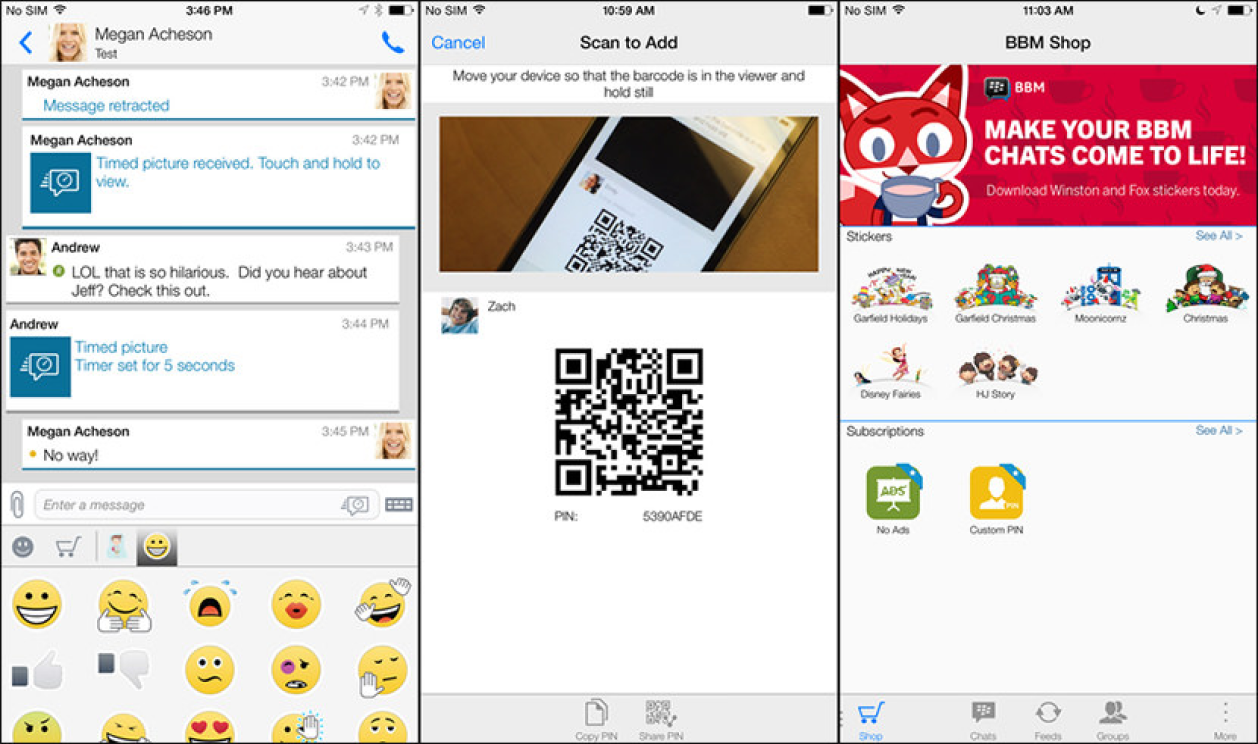
\includegraphics[width=\linewidth]{bilder/research pic/blackberry-messenger-live-free.png}
                                                                                        & \textbf{Blackberry Messenger Live}\newline
    Zuerst haben wir uns umgeschaut und nach Chatfenstern gesucht. Hier haben wir uns die Austauschung von Sprechblasen angeschaut
    und deren Ausrichtung.                                                                                                           \\
    Bildquelle:\cite{blackberry} \newline                                                                                            \\
    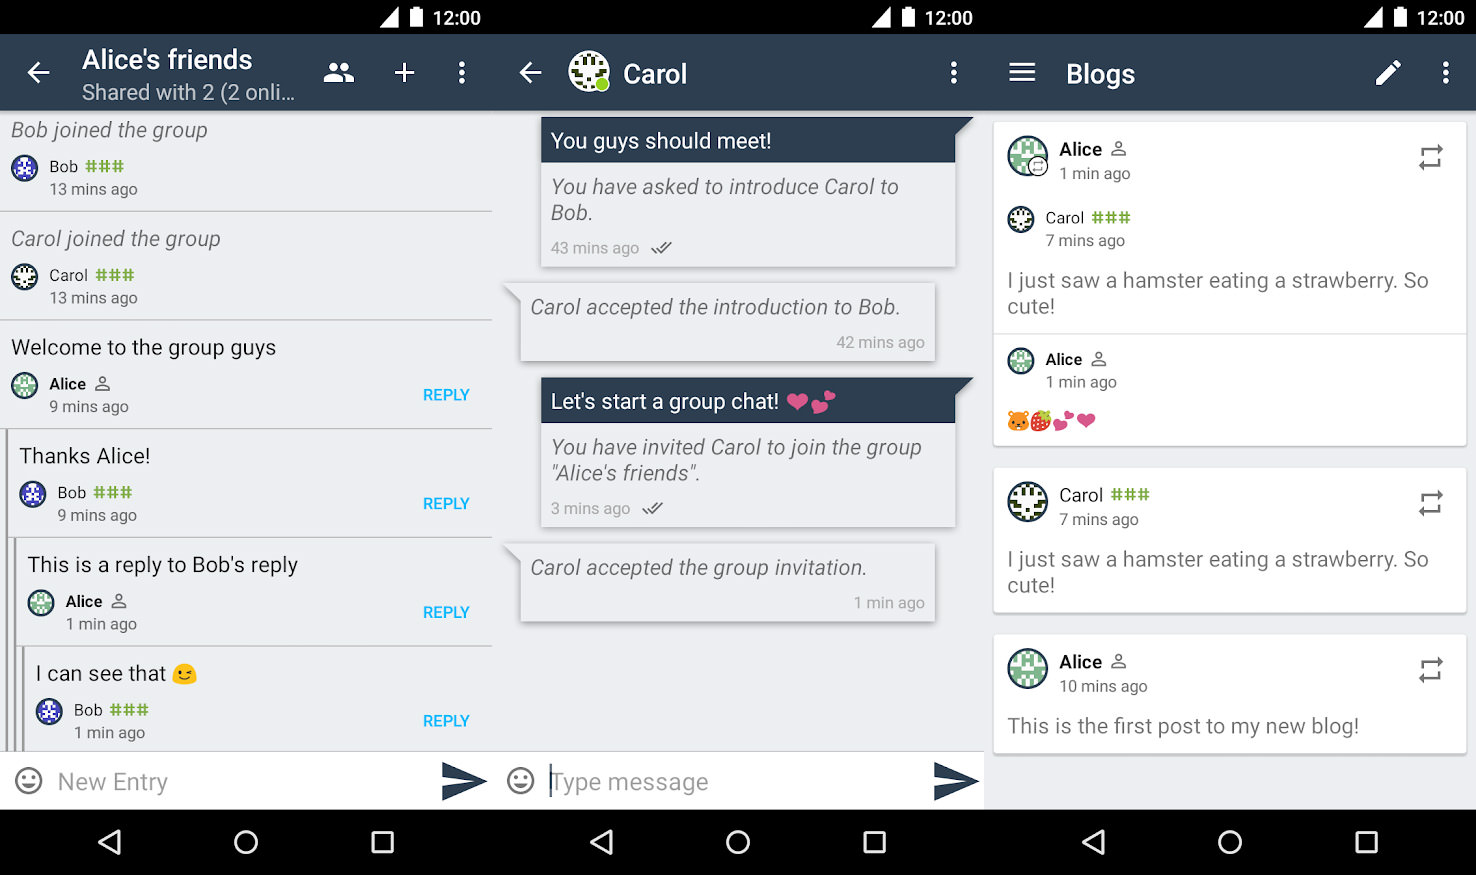
\includegraphics[width=\linewidth]{bilder/research pic/briar.jpg}
                                                                                        & \textbf{Briar} \newline
    In diesem Beispiel haben wir uns wieder das Chatfenster und die verschiedenen Symbole angeschaut.
    Wie das Editierbutton oder das Hinzufügebutton.                                                                                  \\
    Bildquelle:\cite{briar} \newline                                                                                                 \\
    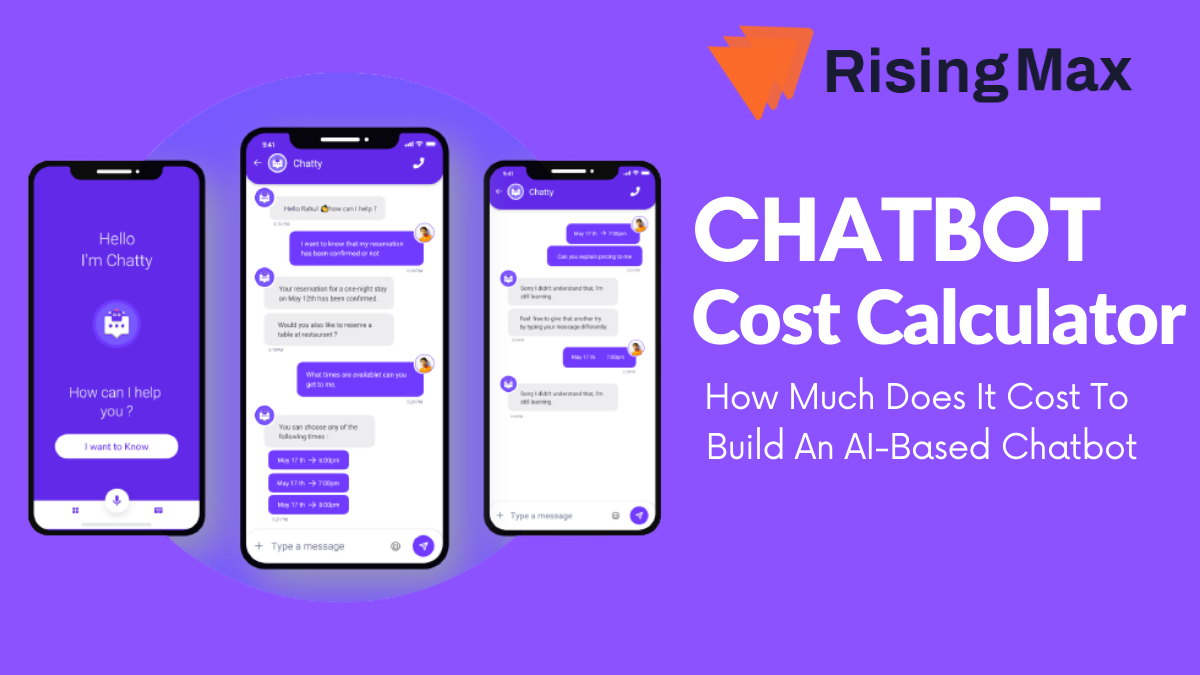
\includegraphics[width=\linewidth]{bilder/research pic/chatbot-cost-calculator.png} & \textbf{CHATBOT Cost Calculator} \newline
    Hier haben wir uns ein ChatBot-Fenster angeschaut und dabei die Icons und die
    verschiedenen Elemente angeschaut, wie den Balken an der Oberseite oder das Sendebutton.                                         \\
    Bildquelle:\cite{chatbotcostcalc} \newline
\end{tabular}

\begin{tabular}{C{6cm}  L{7cm}}
    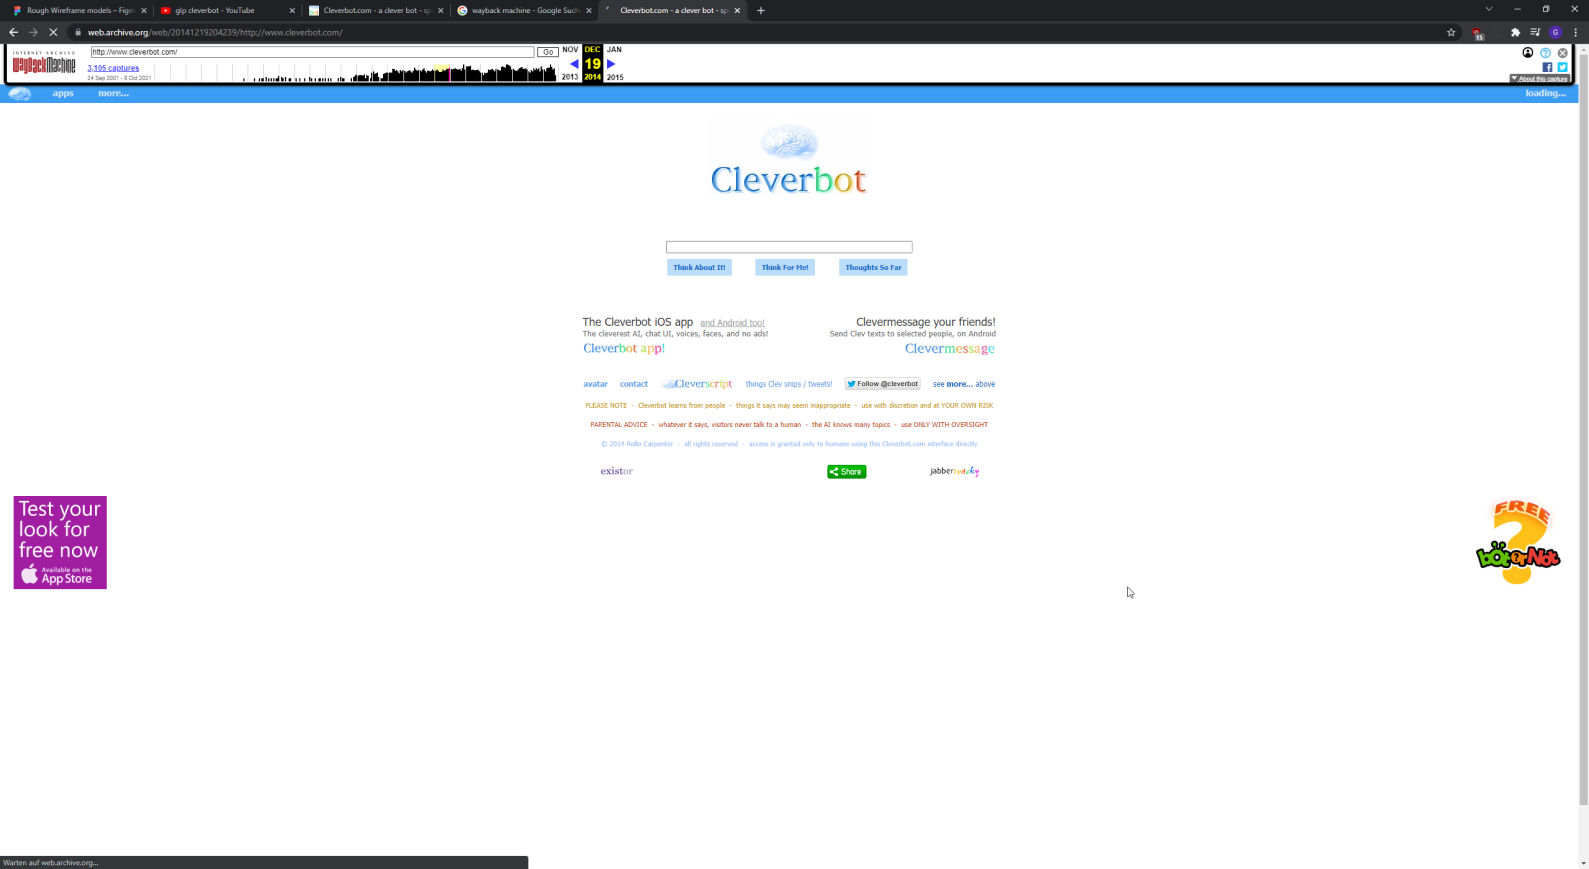
\includegraphics[width=\linewidth]{bilder/research pic/cleverbot.png}                 & \textbf{Cleverbot} \newline
    Diesen Bot haben wir uns genauer angeschaut, weil dieser auch uns bekannt war.                                      \\
    Bildquelle:\cite{cleverbot} \newline
    \\
    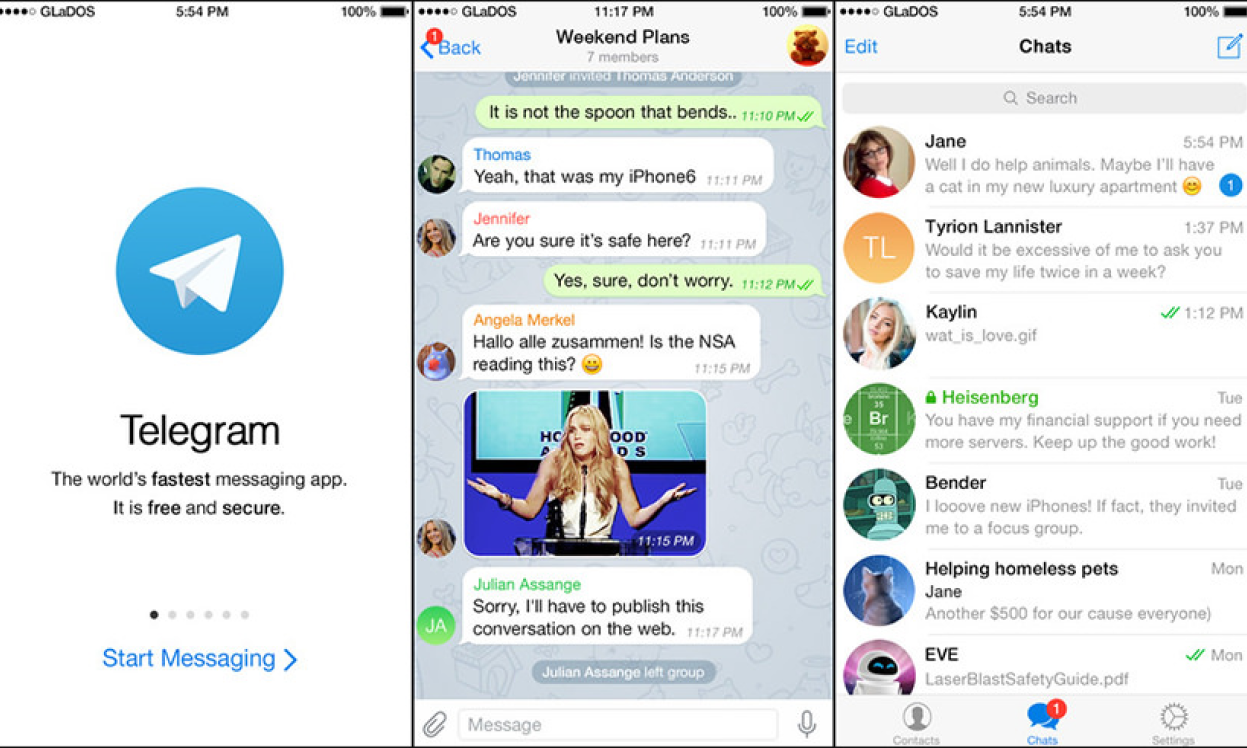
\includegraphics[width=\linewidth]{bilder/research pic/Telegram pic.png}              & \textbf{Telegram} \newline
    Telegram haben wir uns wiederrum das Chatfenster und die Icons angeschaut.                                          \\
    Bildquelle:\cite{telegrambild} \newline
    \\
    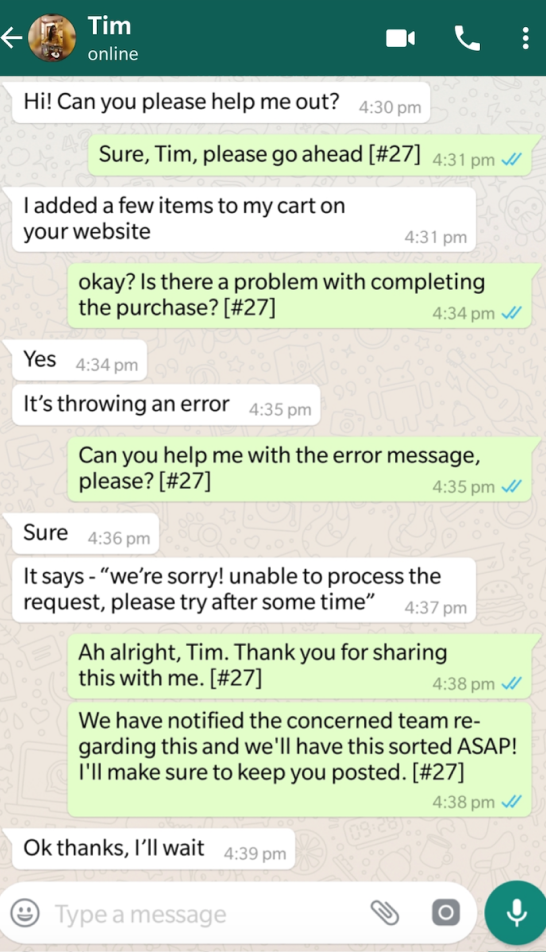
\includegraphics[width=\linewidth, height=12cm]{bilder/research pic/Tim Whatsapp.png} & \textbf{WhatsApp} \newline
    Hier haben wir uns mehr auf die Ausrichtungen des CHatfensters angeschaut und wie die Sprechblasen
    ausgerichtet sind. Fast jeder benutzt WhatsApp deswegen haben wir uns die Struktur angeschaut,
    weil diese viele Benutzer bekannt ist.                                                                              \\
    Bildquelle:\cite{timwhatsApp} \newline
\end{tabular}

\newpage


\subsection{Version 2}

Das sind die neuen Entwürfe des UI Designs. In der neuen Version haben wir uns auf die
feineren Elemente konzentriert und uns sogar eine mobile Versionen ausgedacht, weil wir
unbedingt "mobilefirst" Programmieren möchten.
\\

\begin{tabular}{C{6cm}  L{7cm}}
    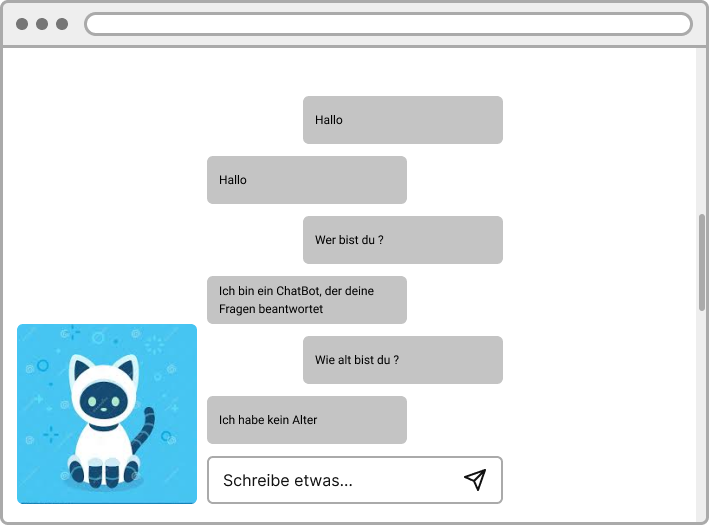
\includegraphics[width=\linewidth]{bilder/new vers. UI Design/WebChat/WebChat.png}                      & \textbf{Webchat} \newline
    Hier haben wir einen Beispielchat mit dem Bot dargestellt. In diesem Beispiel haben wir ein
    Basisgespräch geführt.                                                                                                                                      \\
    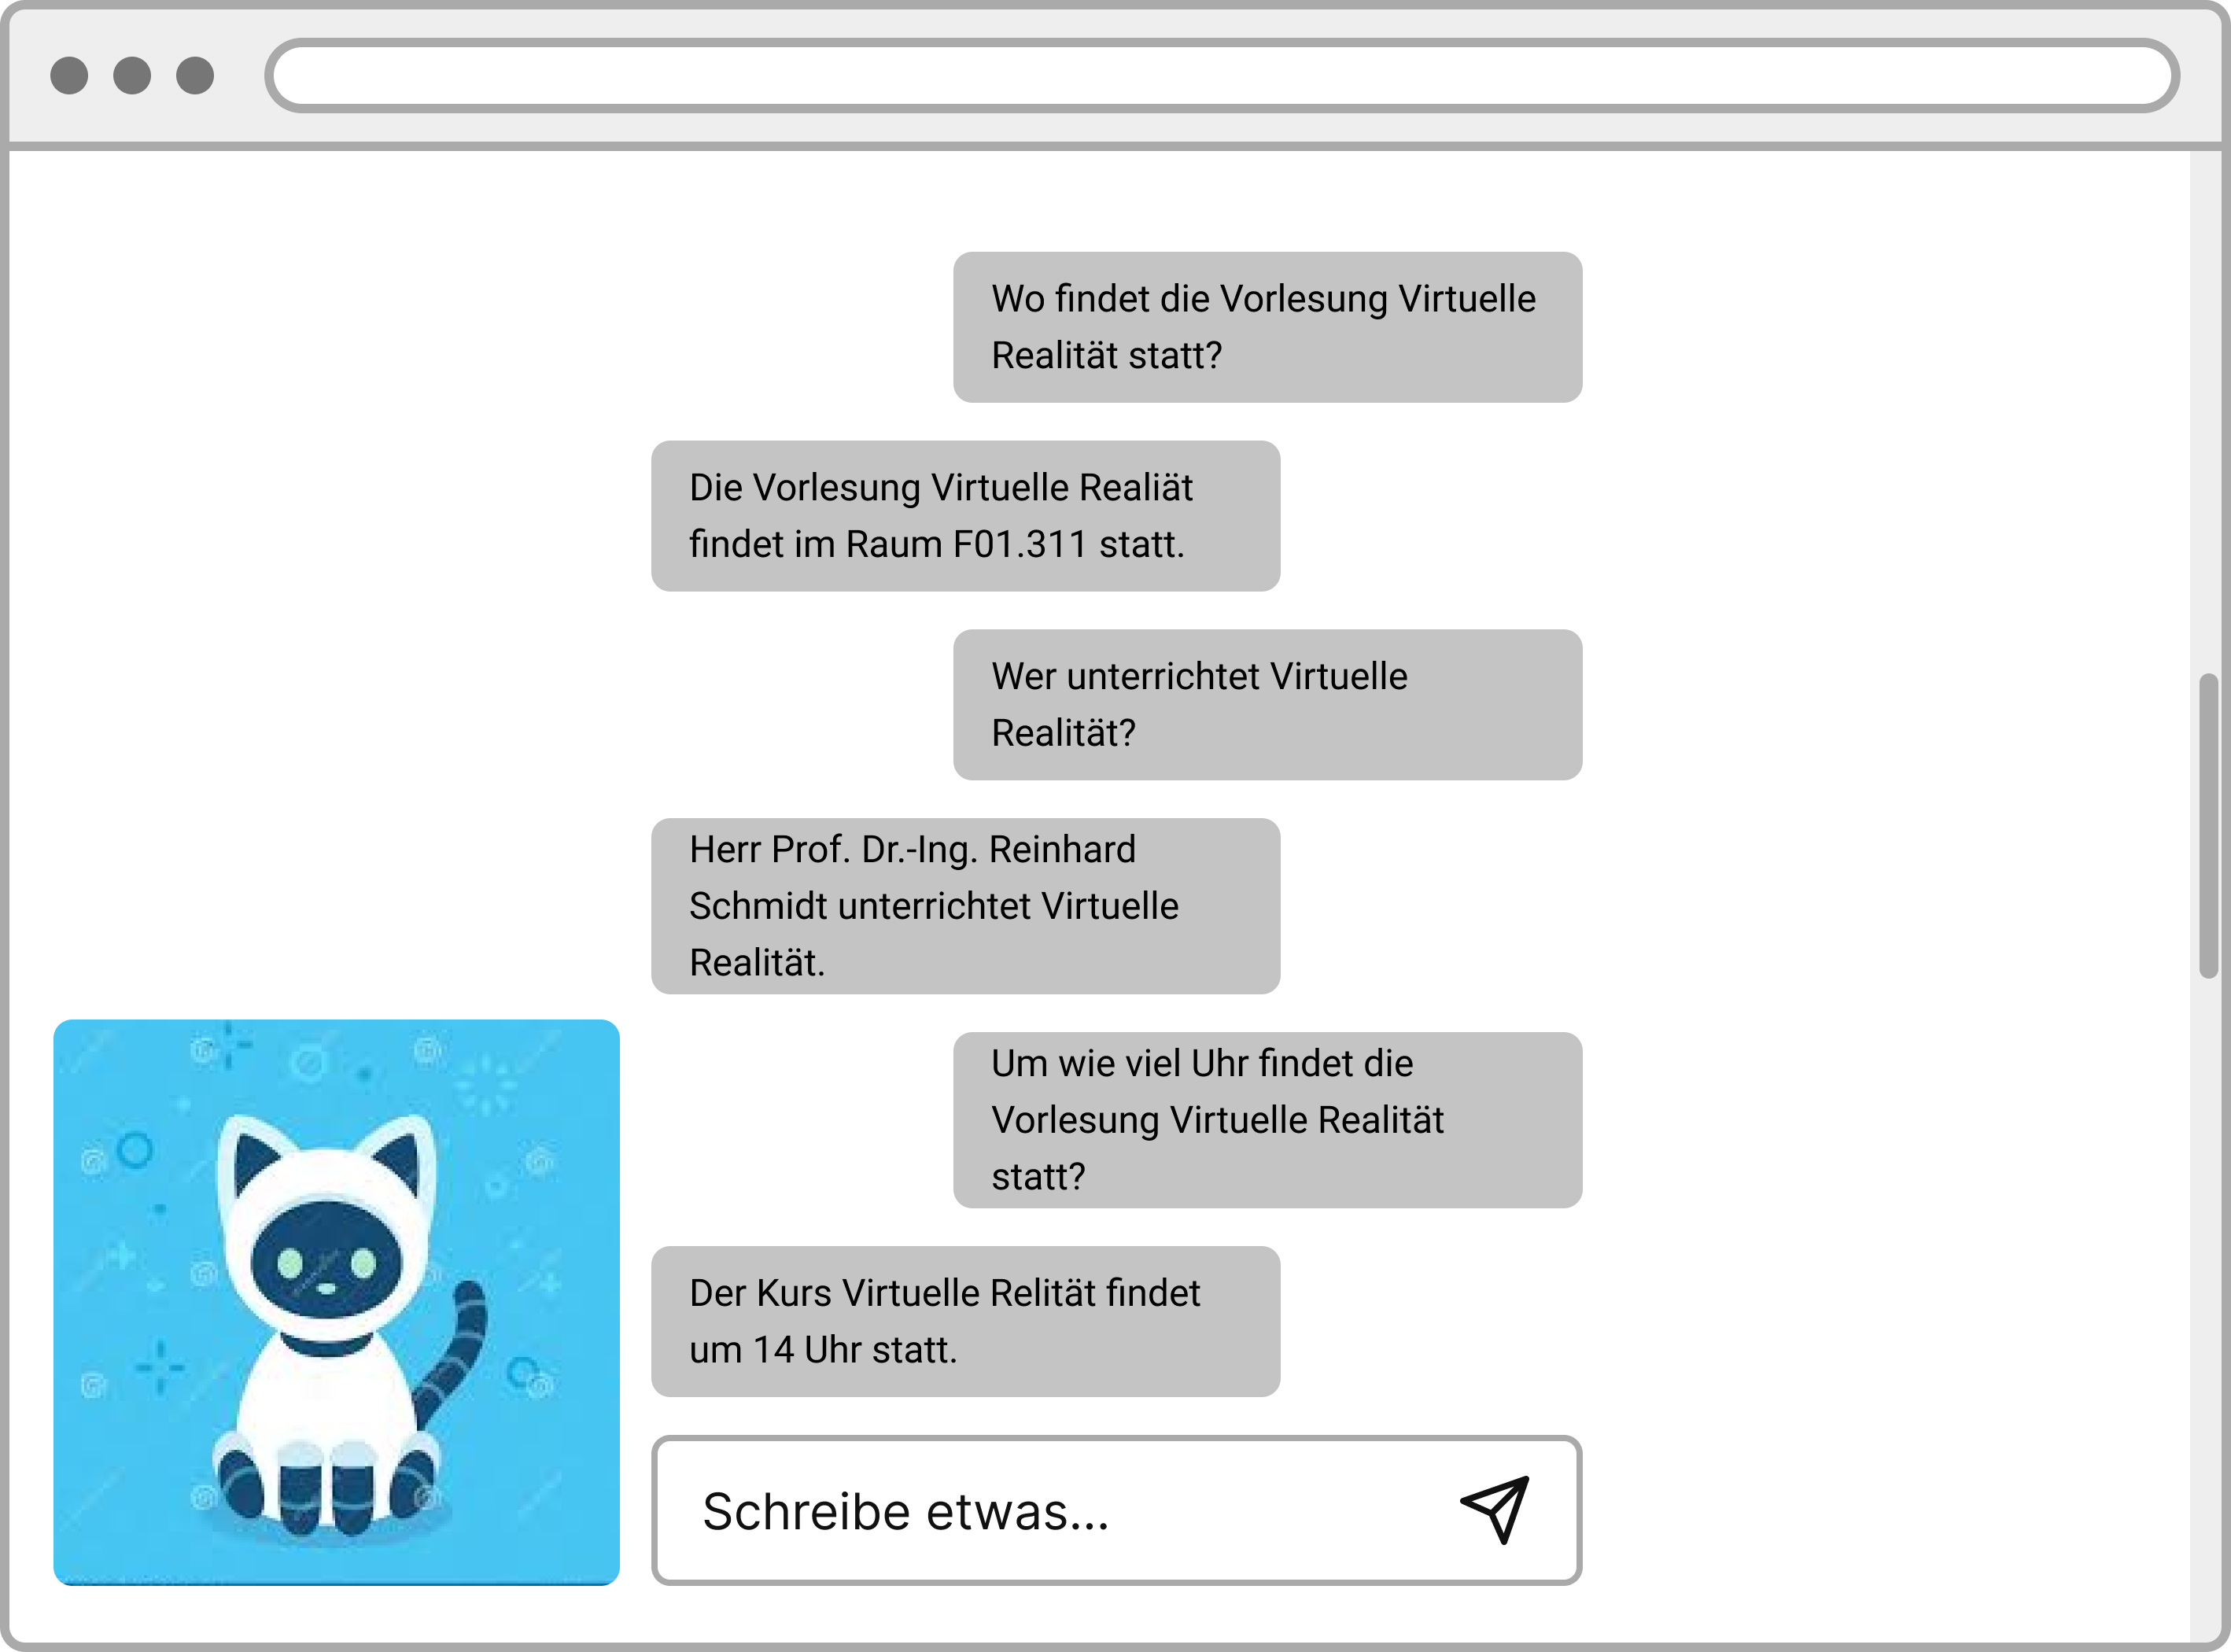
\includegraphics[width=\linewidth]{bilder/new vers. UI Design/WebChat/WebChat Hochschule.png}           & \textbf{Webchat mit der Hochschuldomäne} \newline
    Diesmal haben wir konkrete Hochschulfragen gestellt und die Hochschuldomäne dargestellt.                                                                    \\
    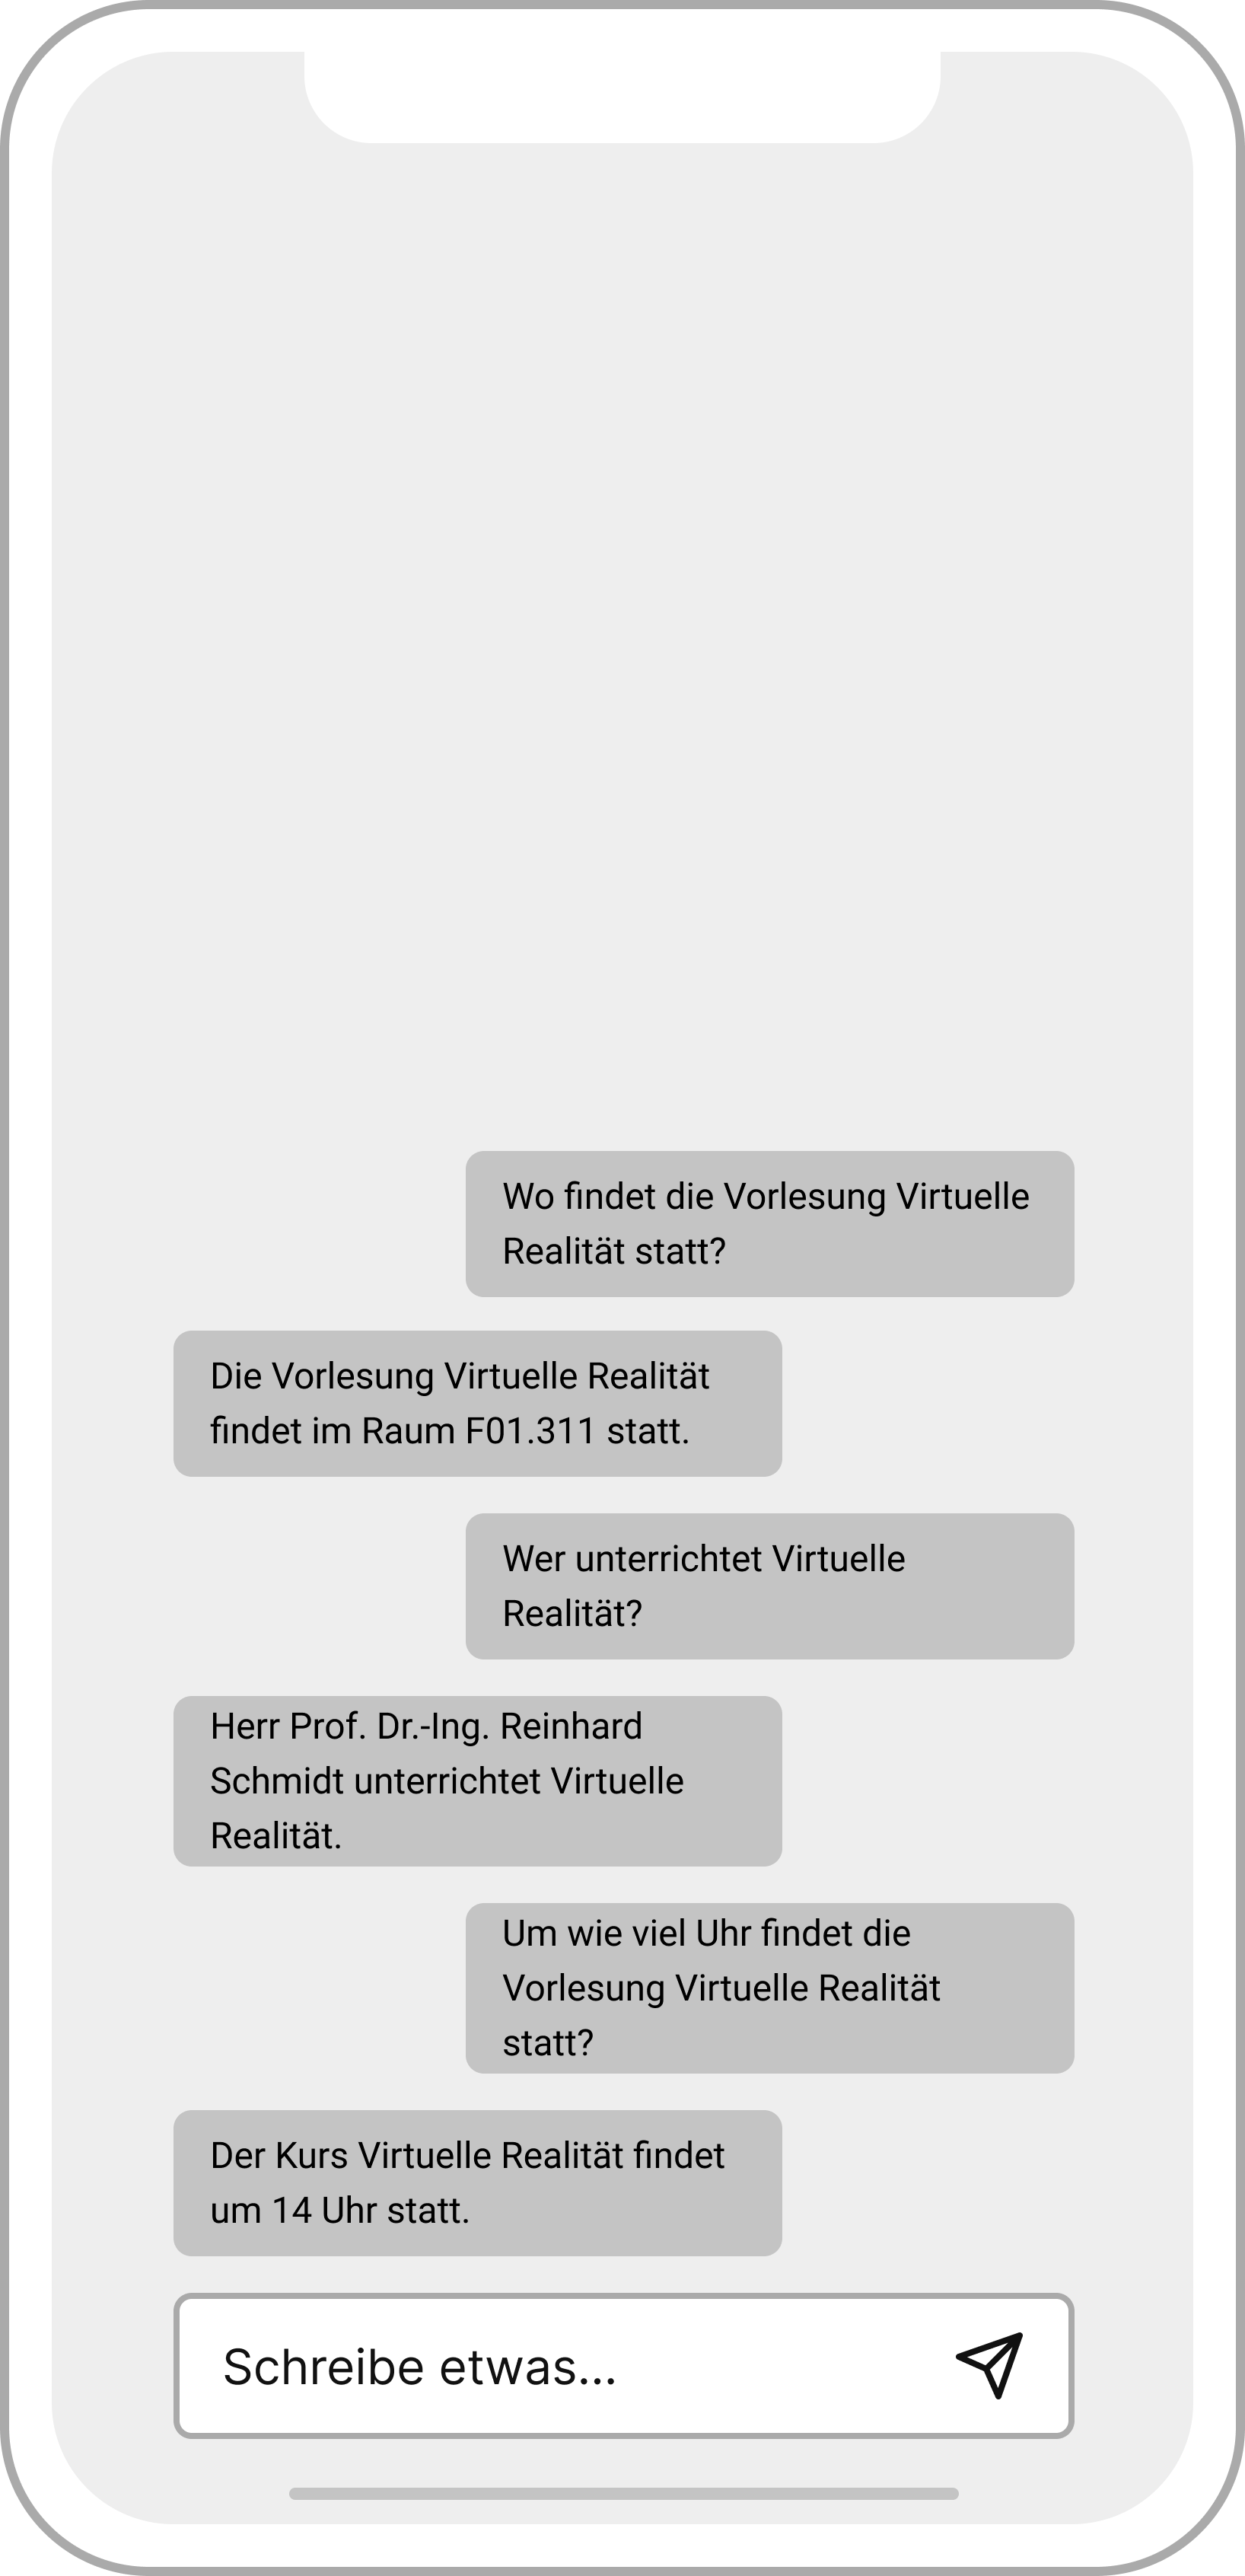
\includegraphics[width=5cm,height=8.5cm]{bilder/new vers. UI Design/WebChat/mobile Version Webchat.png} & \textbf{Webchat als mobile Version} \newline
    Dies ist die mobile Version des Webchats. Wir haben die Darstellung so einfach wie möglich dargestellt.
    Hier haben wir auch die Hochschulbezogenen Fragen gestellt.
\end{tabular}

\begin{tabular}{C{6cm}  L{7cm}}
    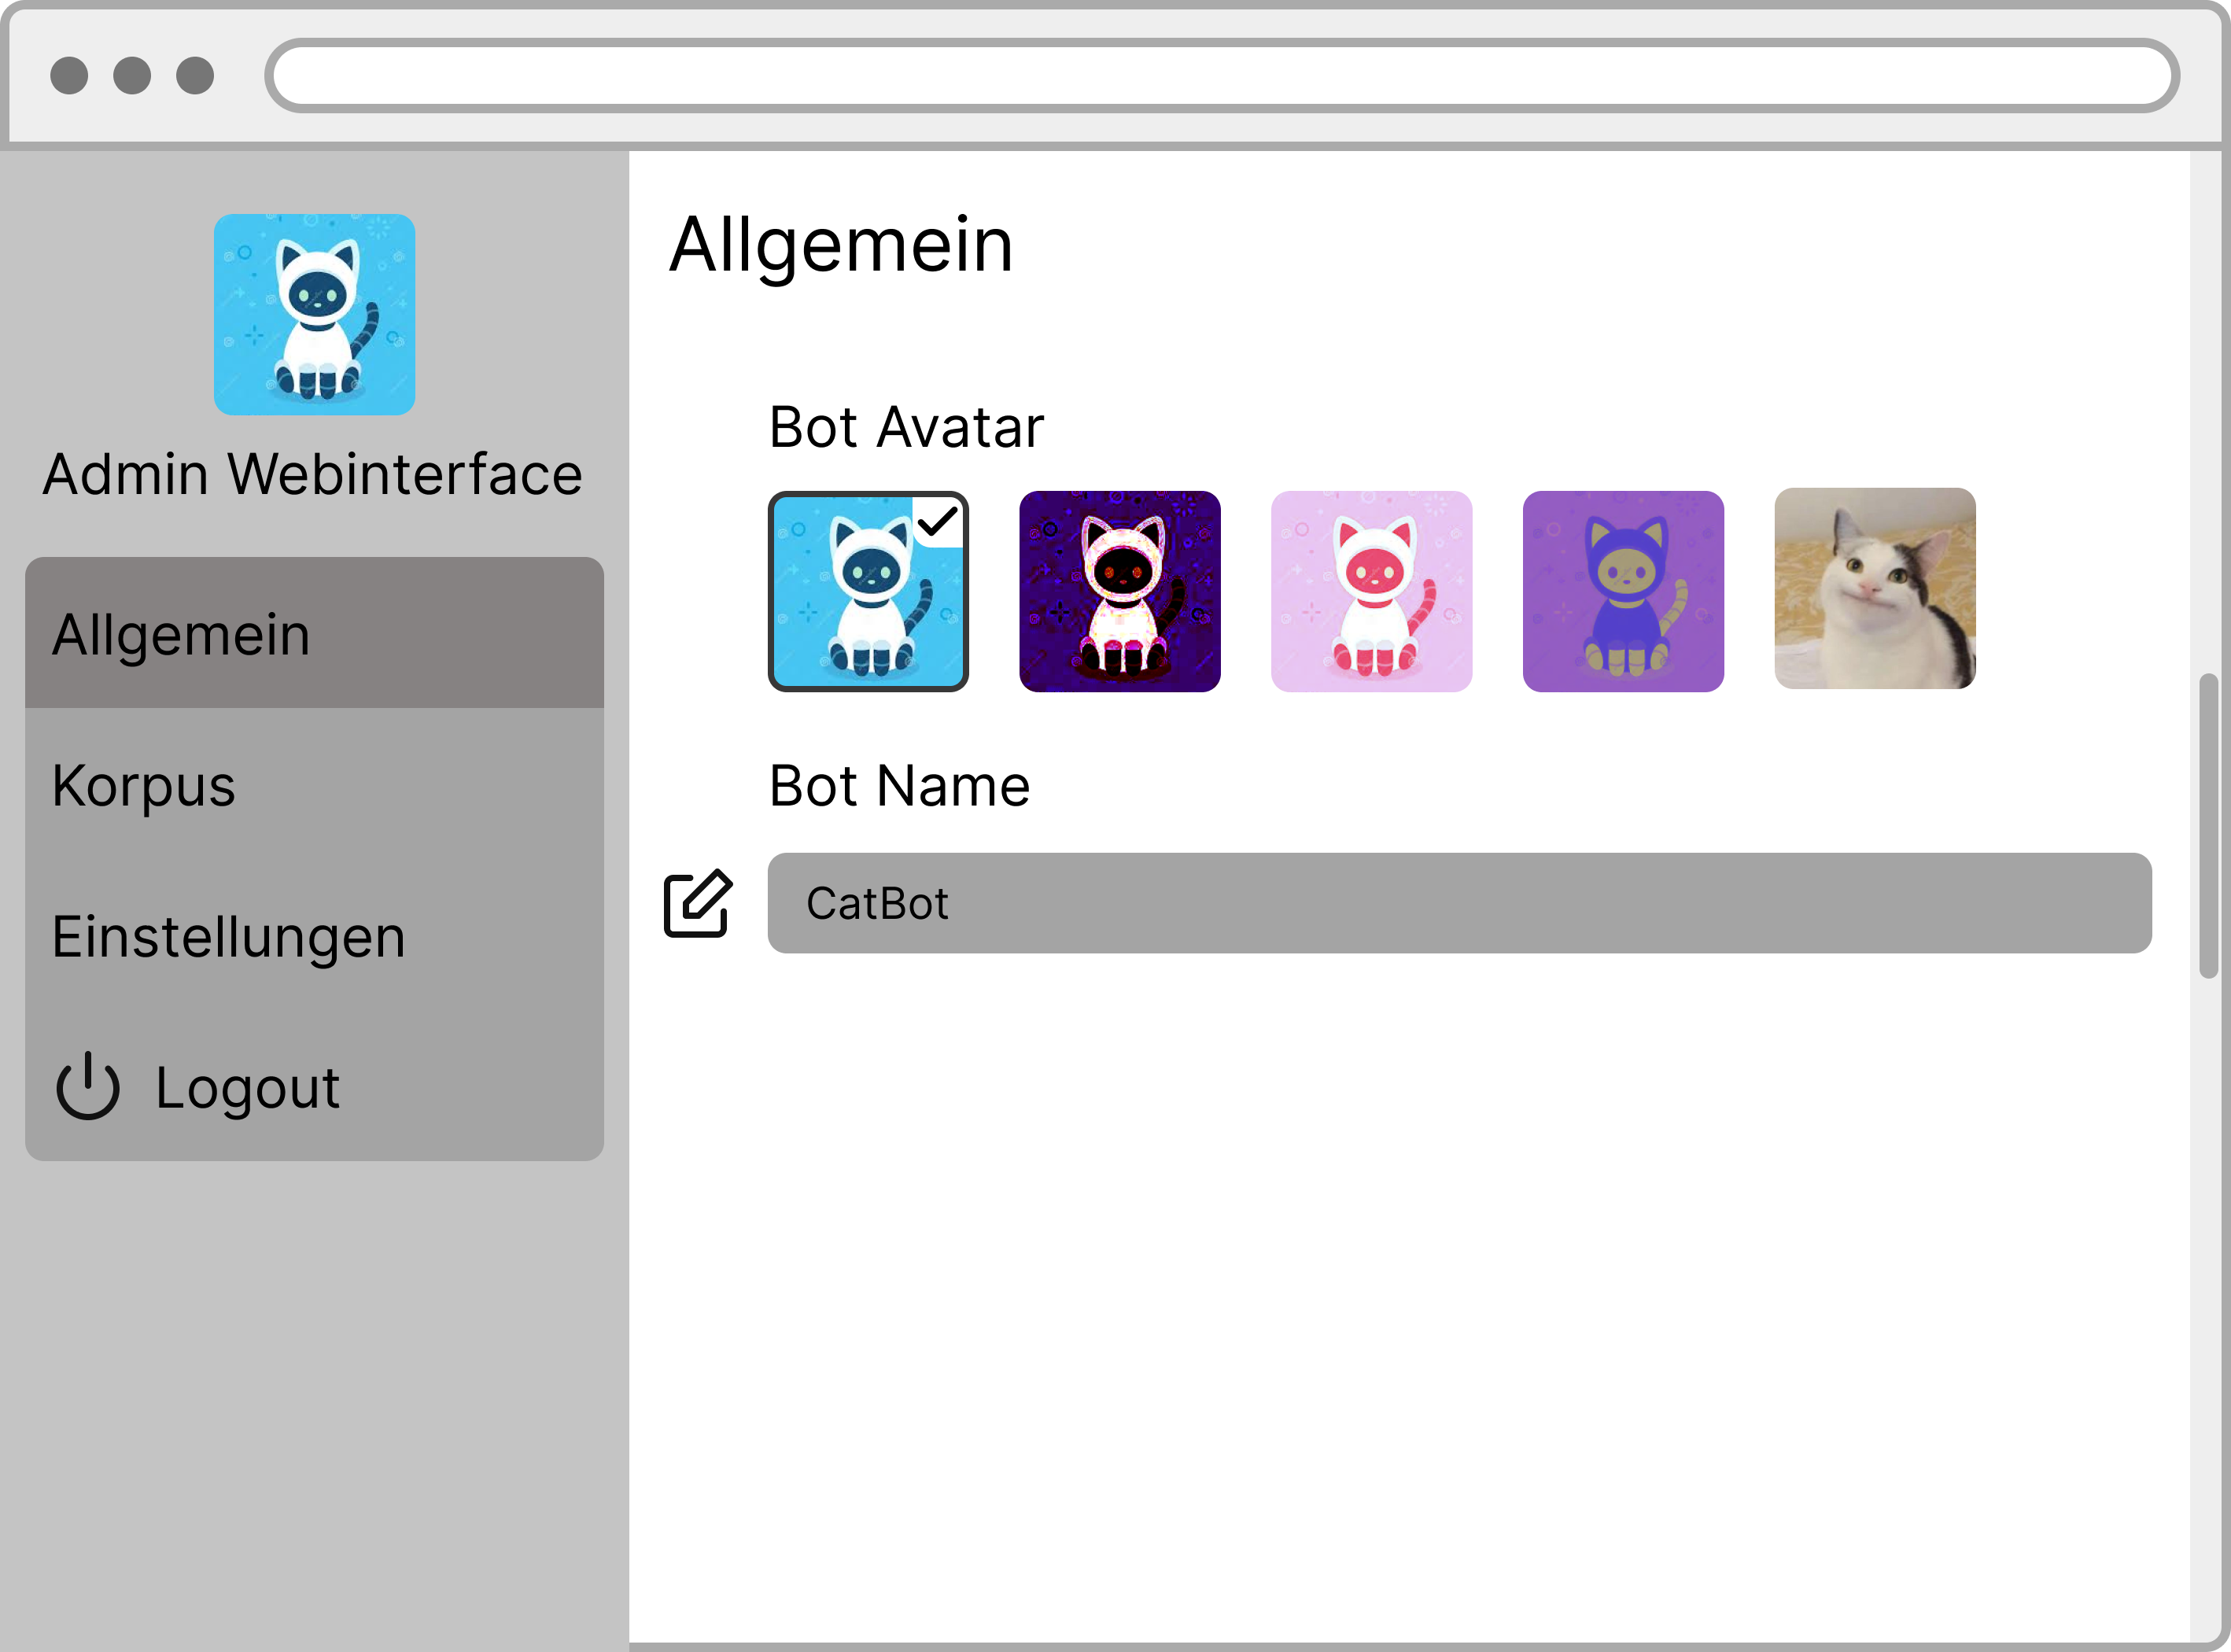
\includegraphics[width=\linewidth]{bilder/new vers. UI Design/Allgemein/Allgemein.png}                         & \textbf{Admin Webinterface: Allgemein} \newline
    Auf der linken Seite sieht man die Kategorien, die der Admin bearbeiten kann. Im Allgemeinen kann
    der Admin den Bot Avatar wechseln, diese wird dann mit einem Haken gekennzeichnet. Außerdem kann
    der Admin den Bot Namen ändern, indem er den Editierbutton drückt.                                                                                                                   \\
    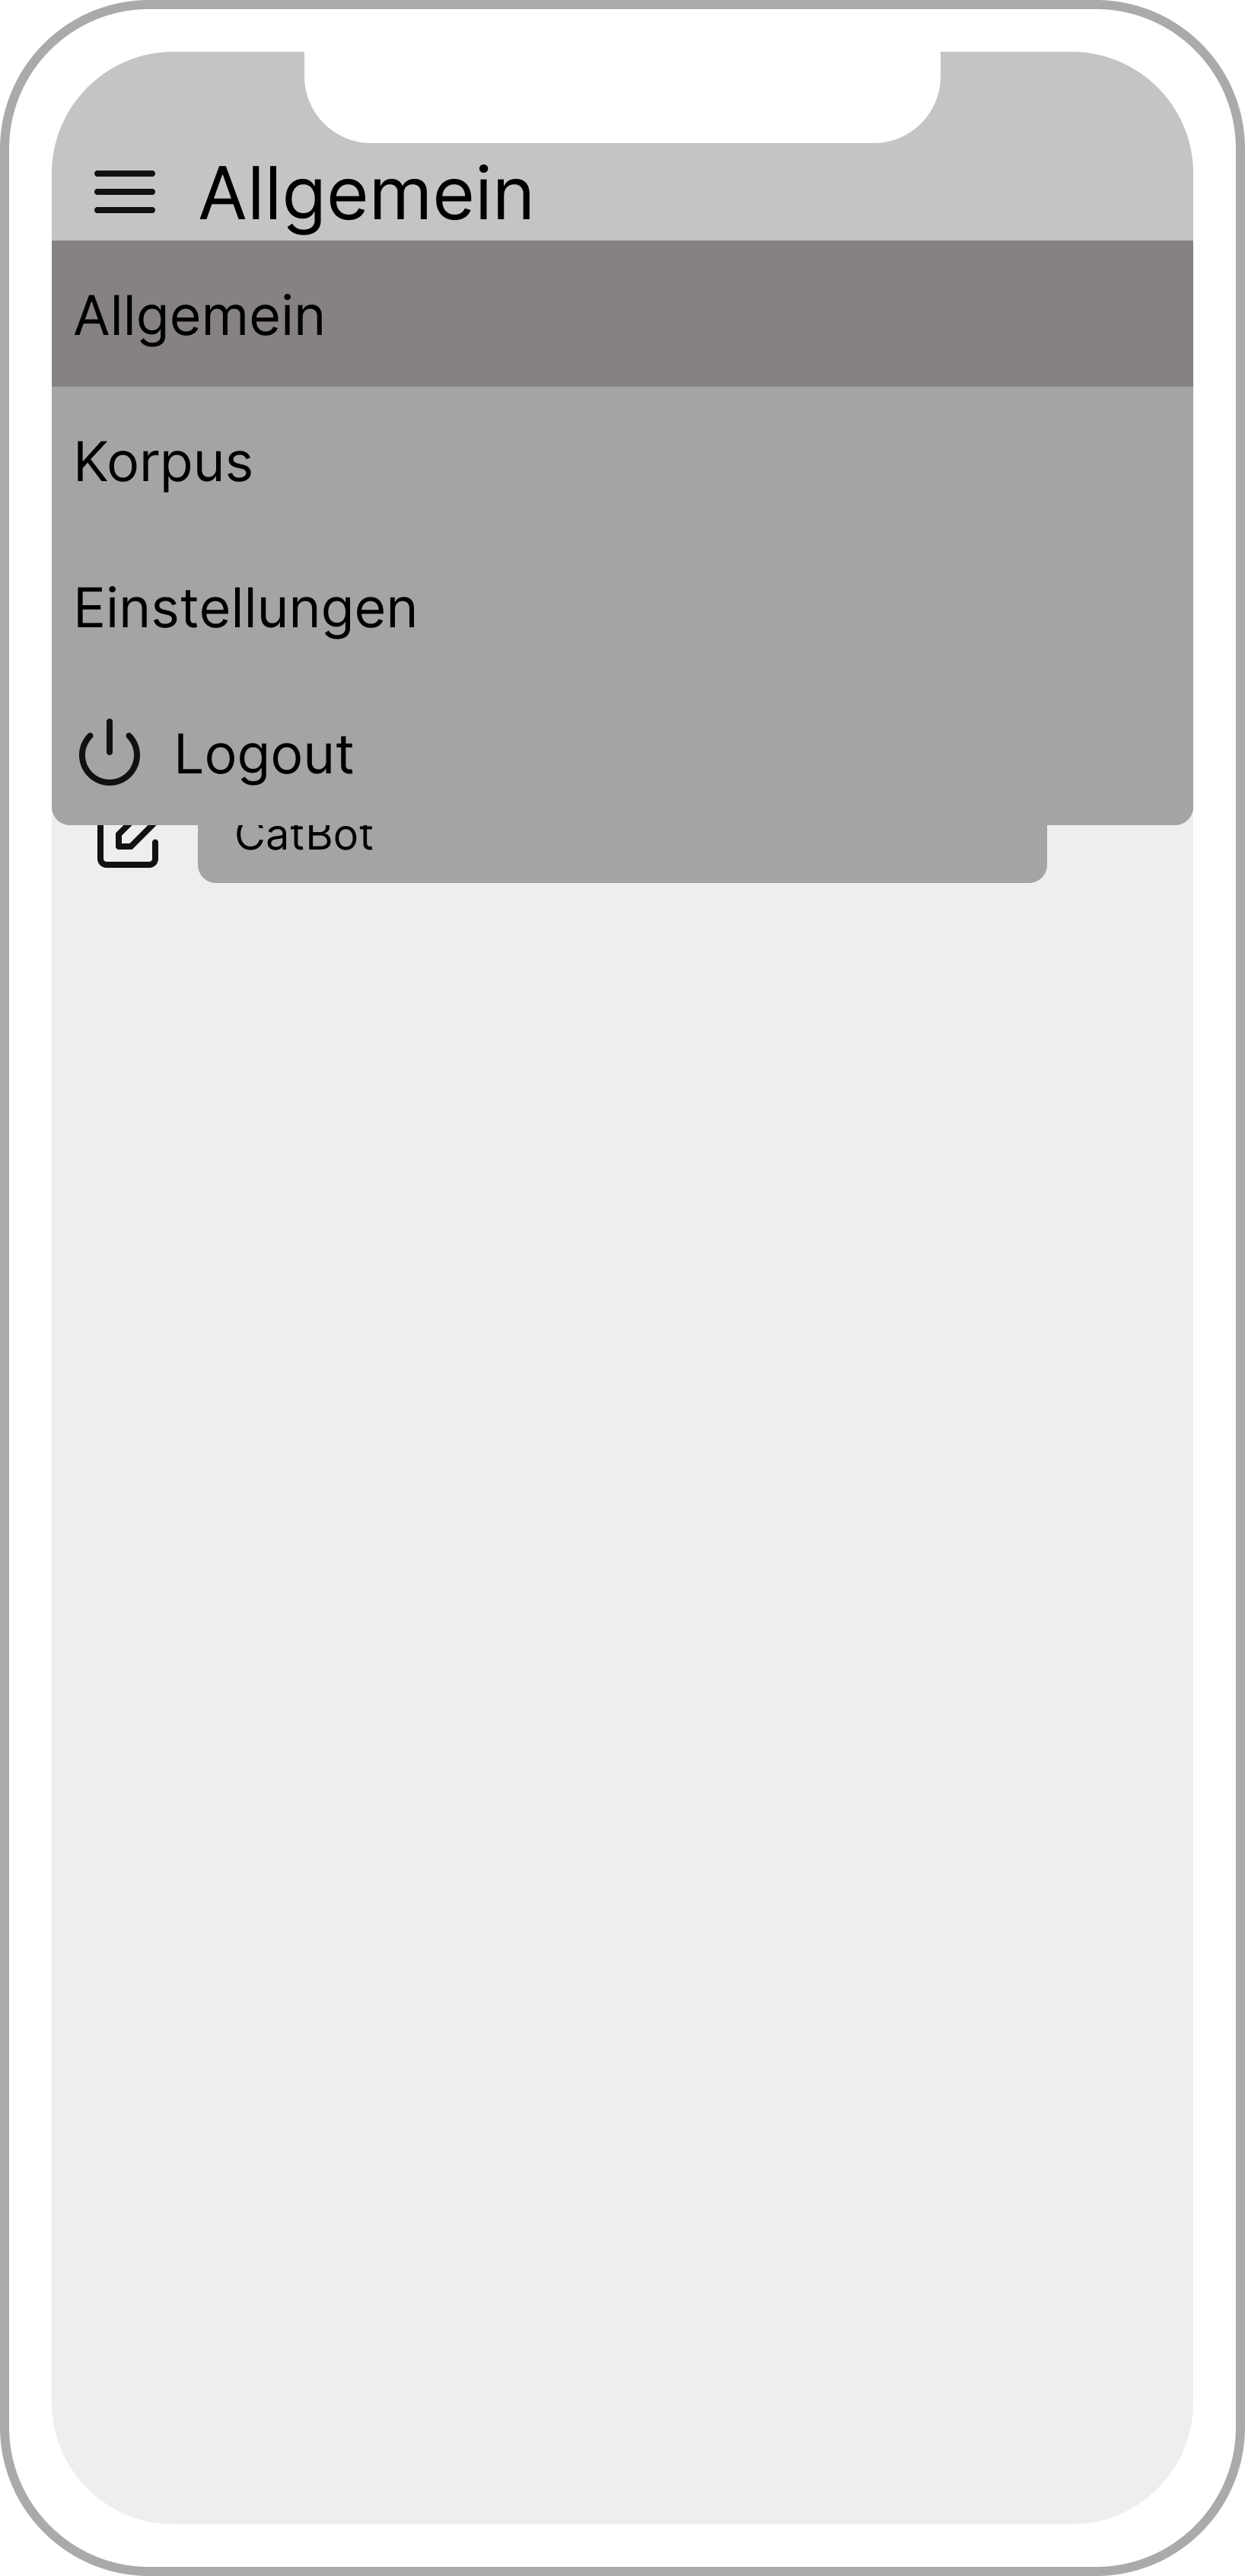
\includegraphics[width=5cm,height=8.5cm]{bilder/new vers. UI Design/Allgemein/iPhone X Allgemein dropdown.png} & \textbf{Admin Webinterface mobil: Allgemein dropdown Menü} \newline
    In der mobilen Version haben wir die Kategorien, die der Admin bearbeiten kann im dropdown Menü dargestellt.                                                                         \\
    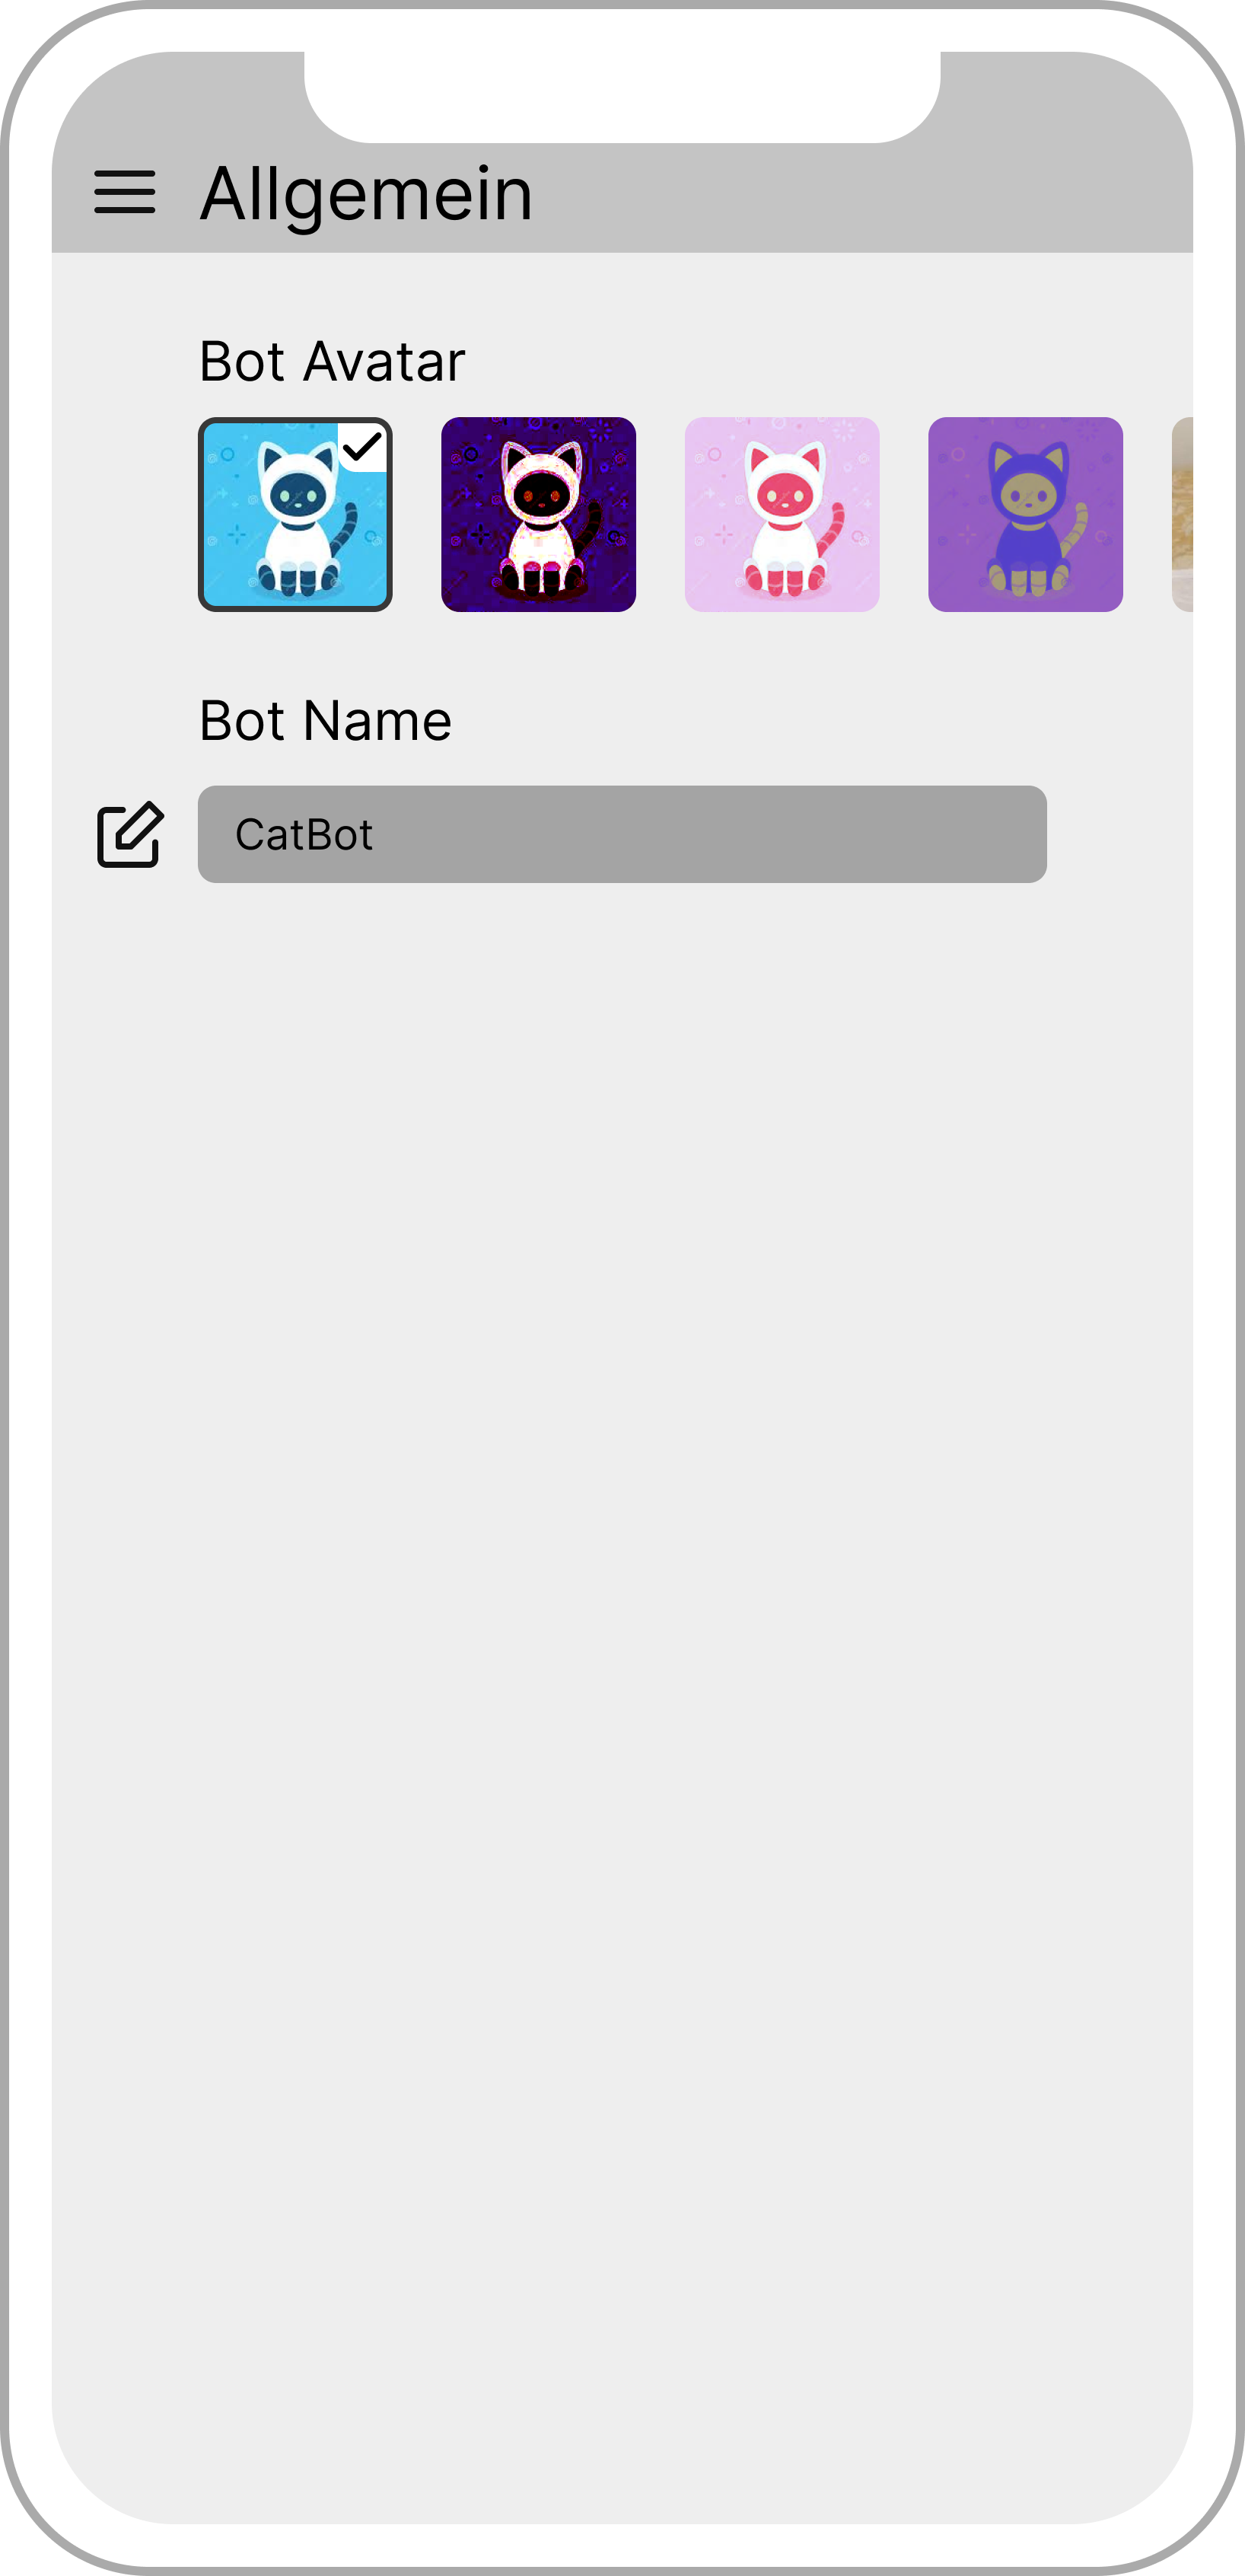
\includegraphics[width=5cm,height=8.5cm]{bilder/new vers. UI Design/Allgemein/iPhone X Allgemein III.png}      & \textbf{Admin Webinterface mobil: Allgemein} \newline
    Die mobile Variante funktioniert genauso wie die Webvariante. Man kann den Bot Avatar wechseln und den
    ChatBot Namen frei bestimmen.
\end{tabular}

\begin{tabular}{C{6cm}  L{7cm}}
    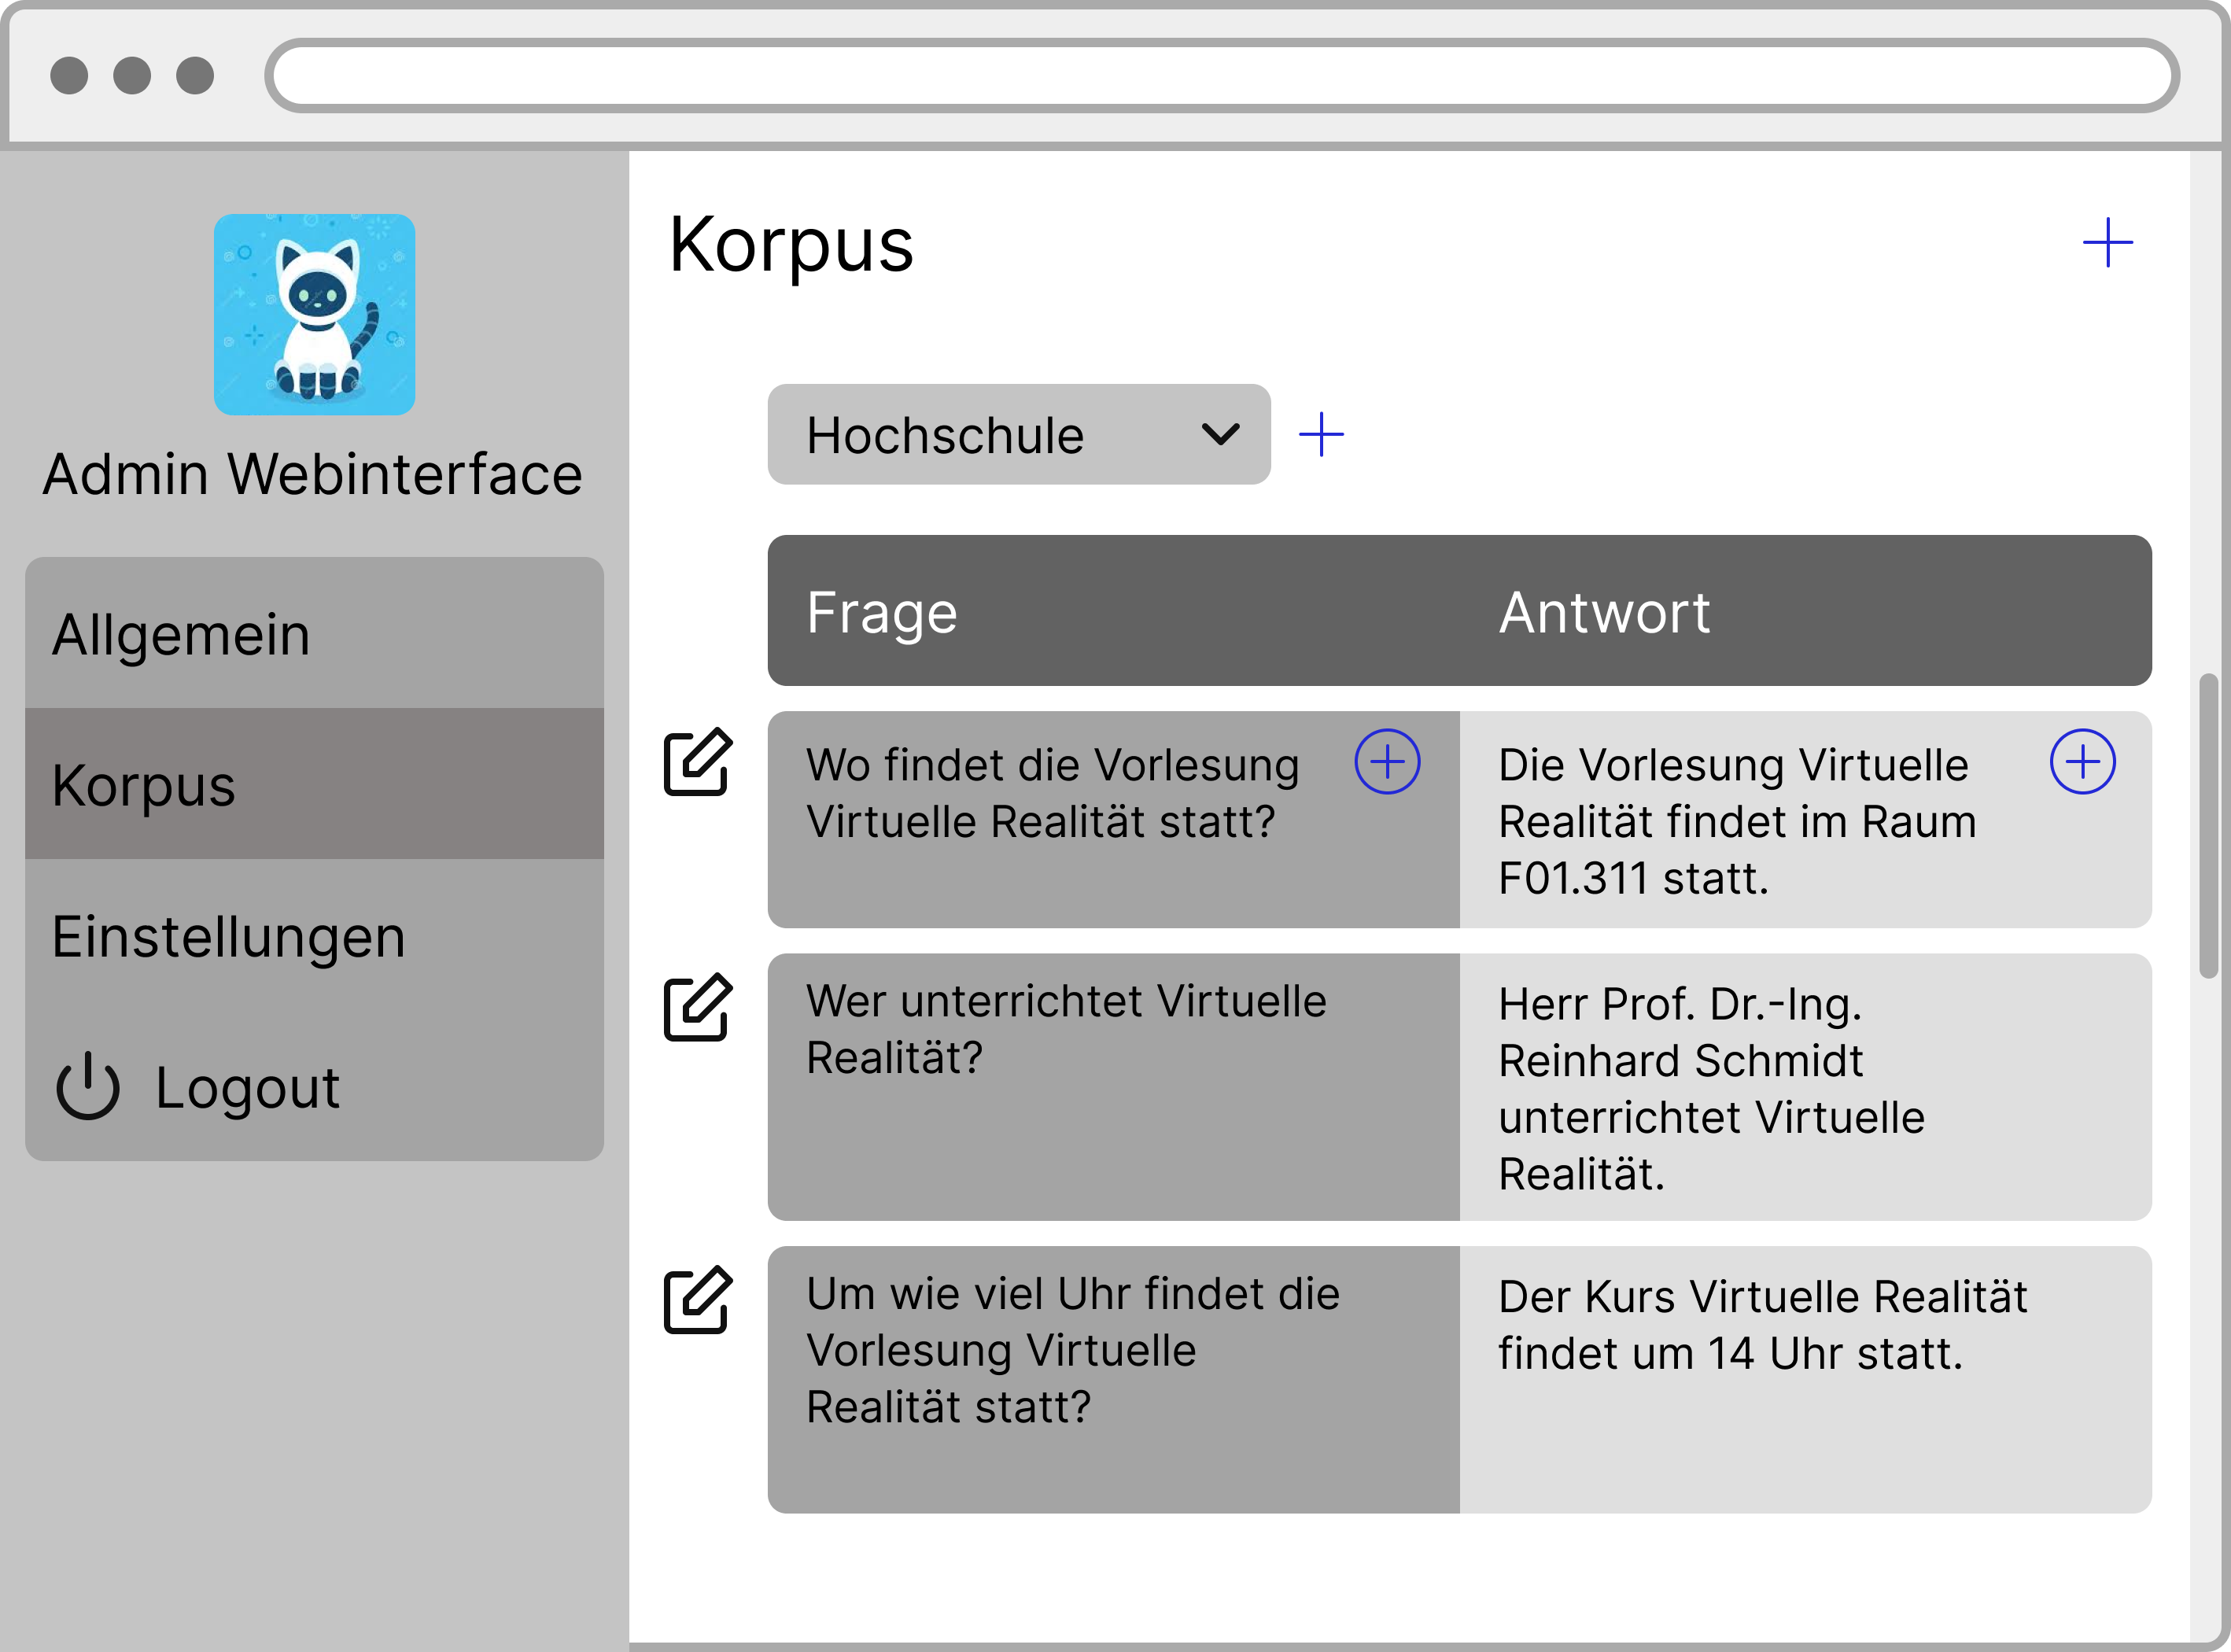
\includegraphics[width=\linewidth]{bilder/new vers. UI Design/Korpus/Admin Interface 00.png} & \textbf{Admin Webinterface: Korpus 00} \newline
    Im Korpus kann der Admin weitere Domänen, Fragen und Antworten einsehen.                                                                       \\
    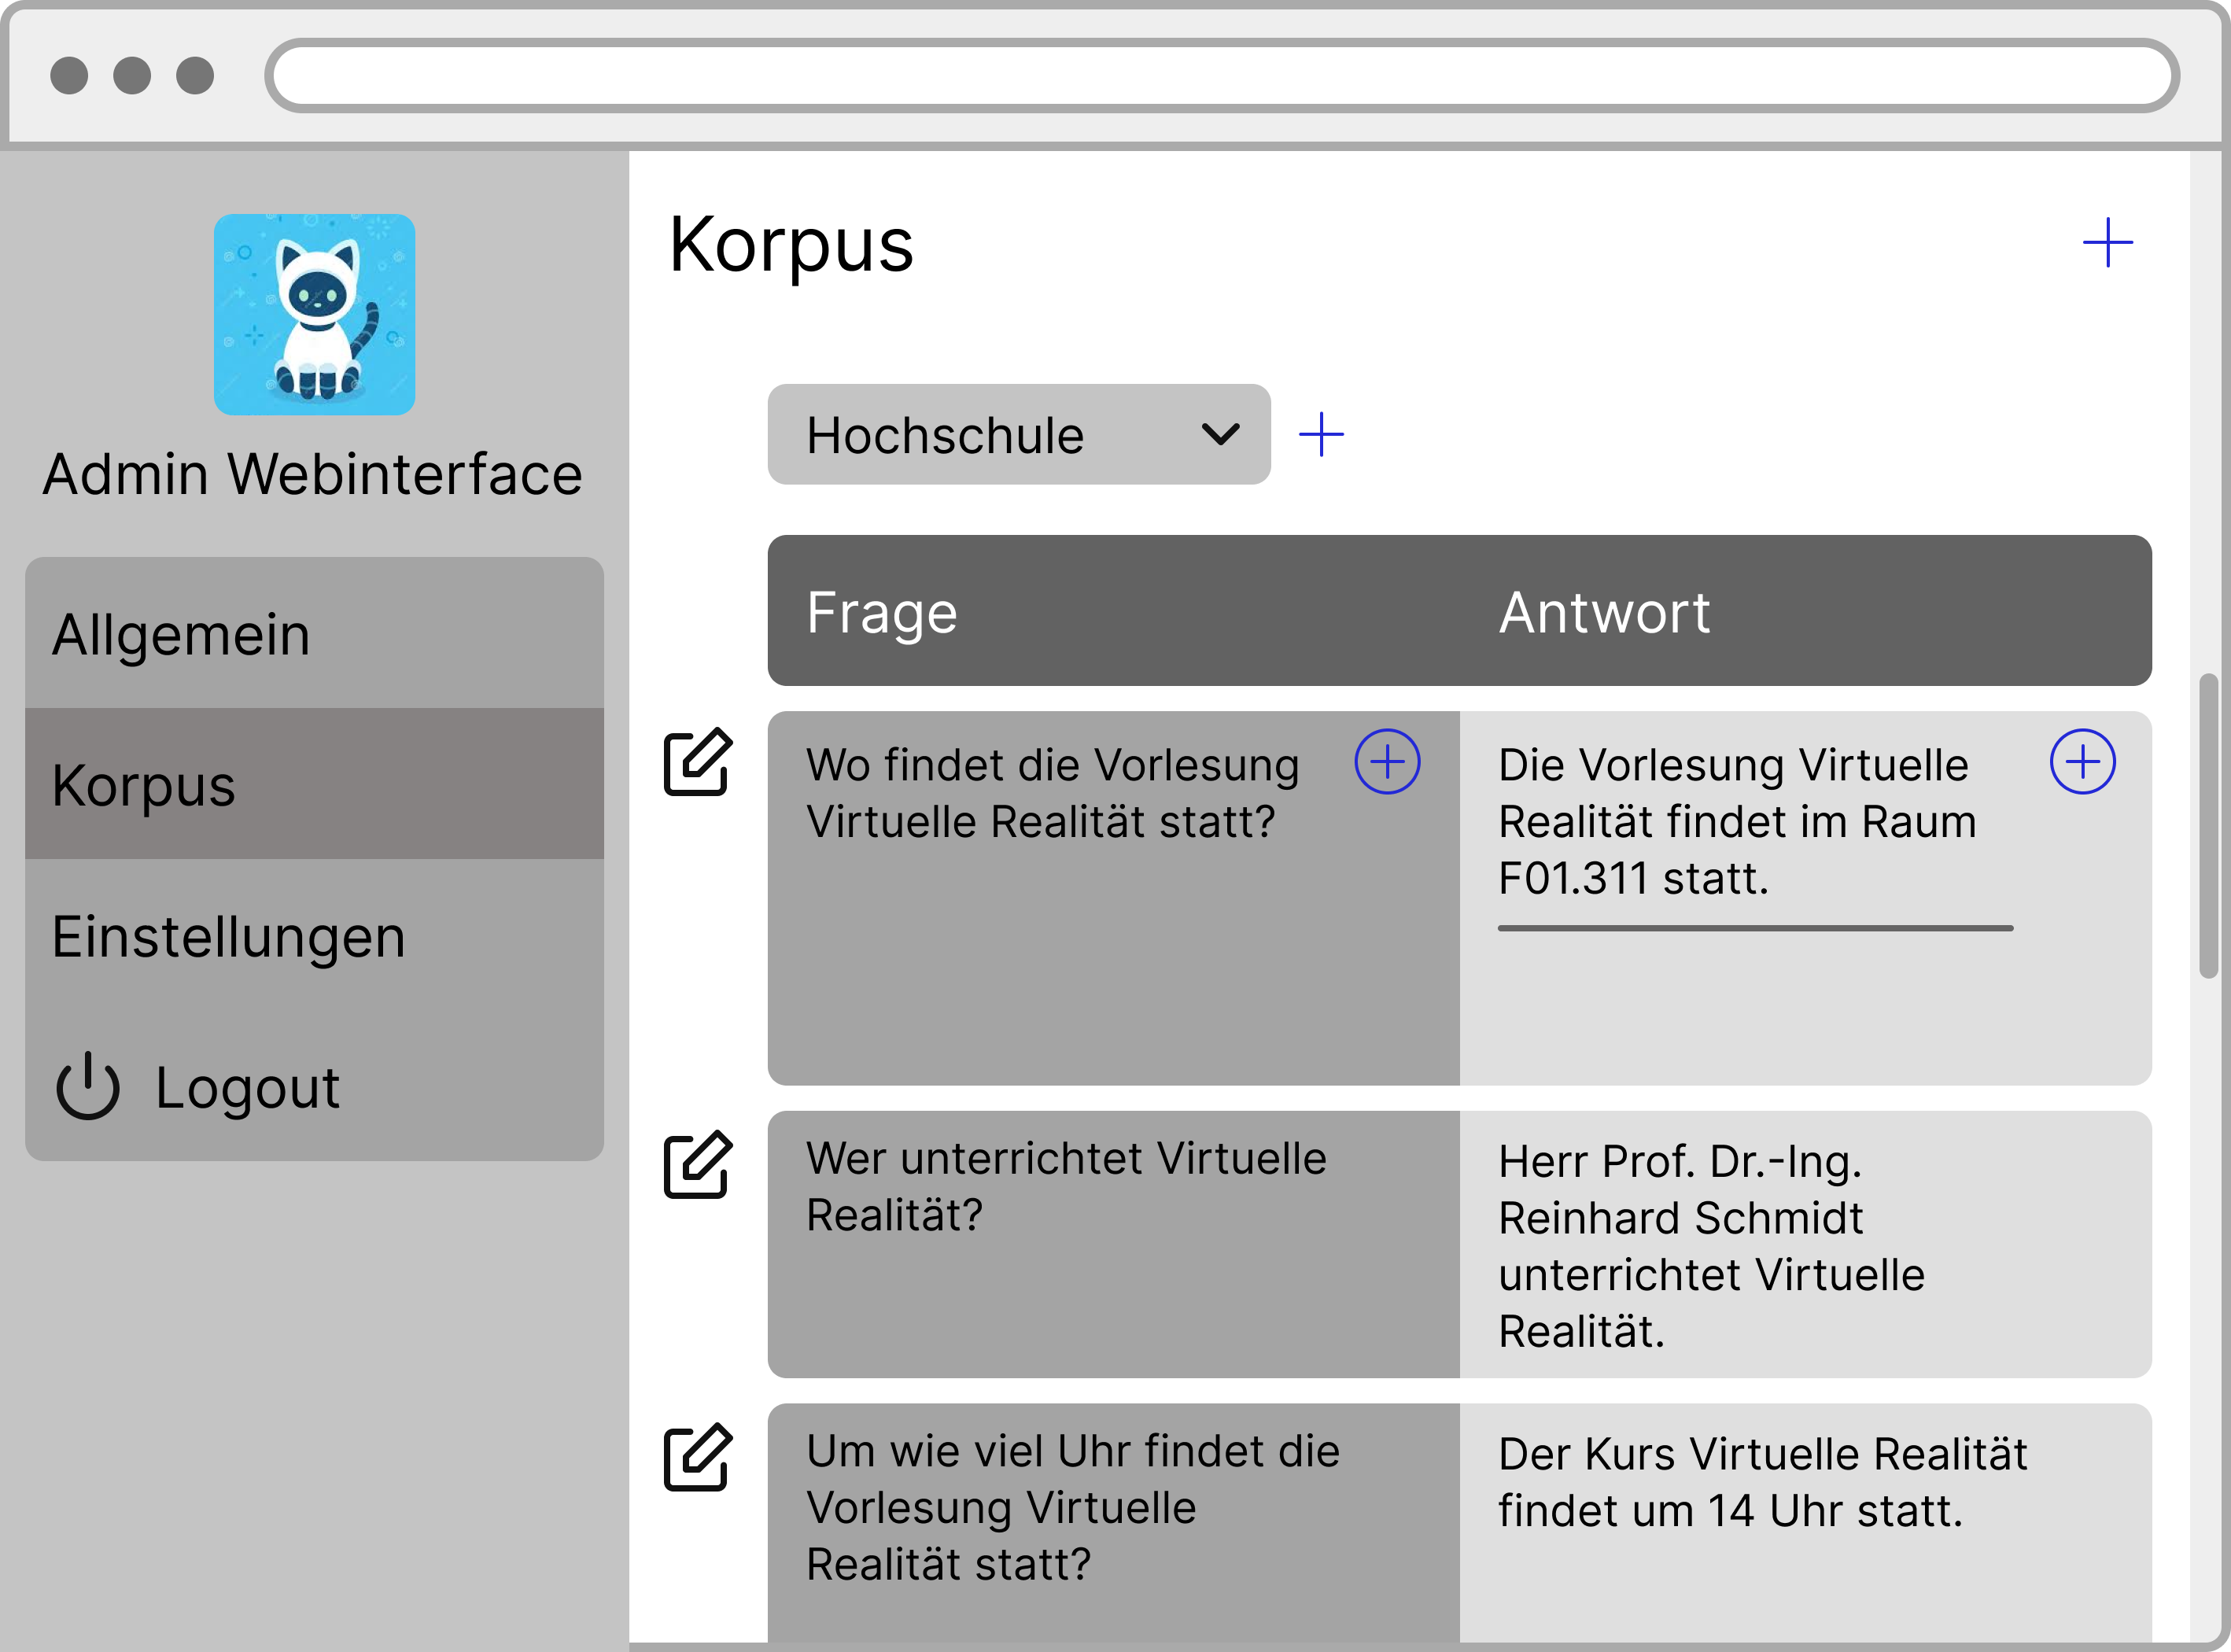
\includegraphics[width=\linewidth]{bilder/new vers. UI Design/Korpus/Admin Interface 01.png} & \textbf{Admin Webinterface: Korpus 01} \newline
    Mit dem Editierbutton kann er Domänen, Fragen und Antworten hinzufügen und entfernen.                                                          \\
    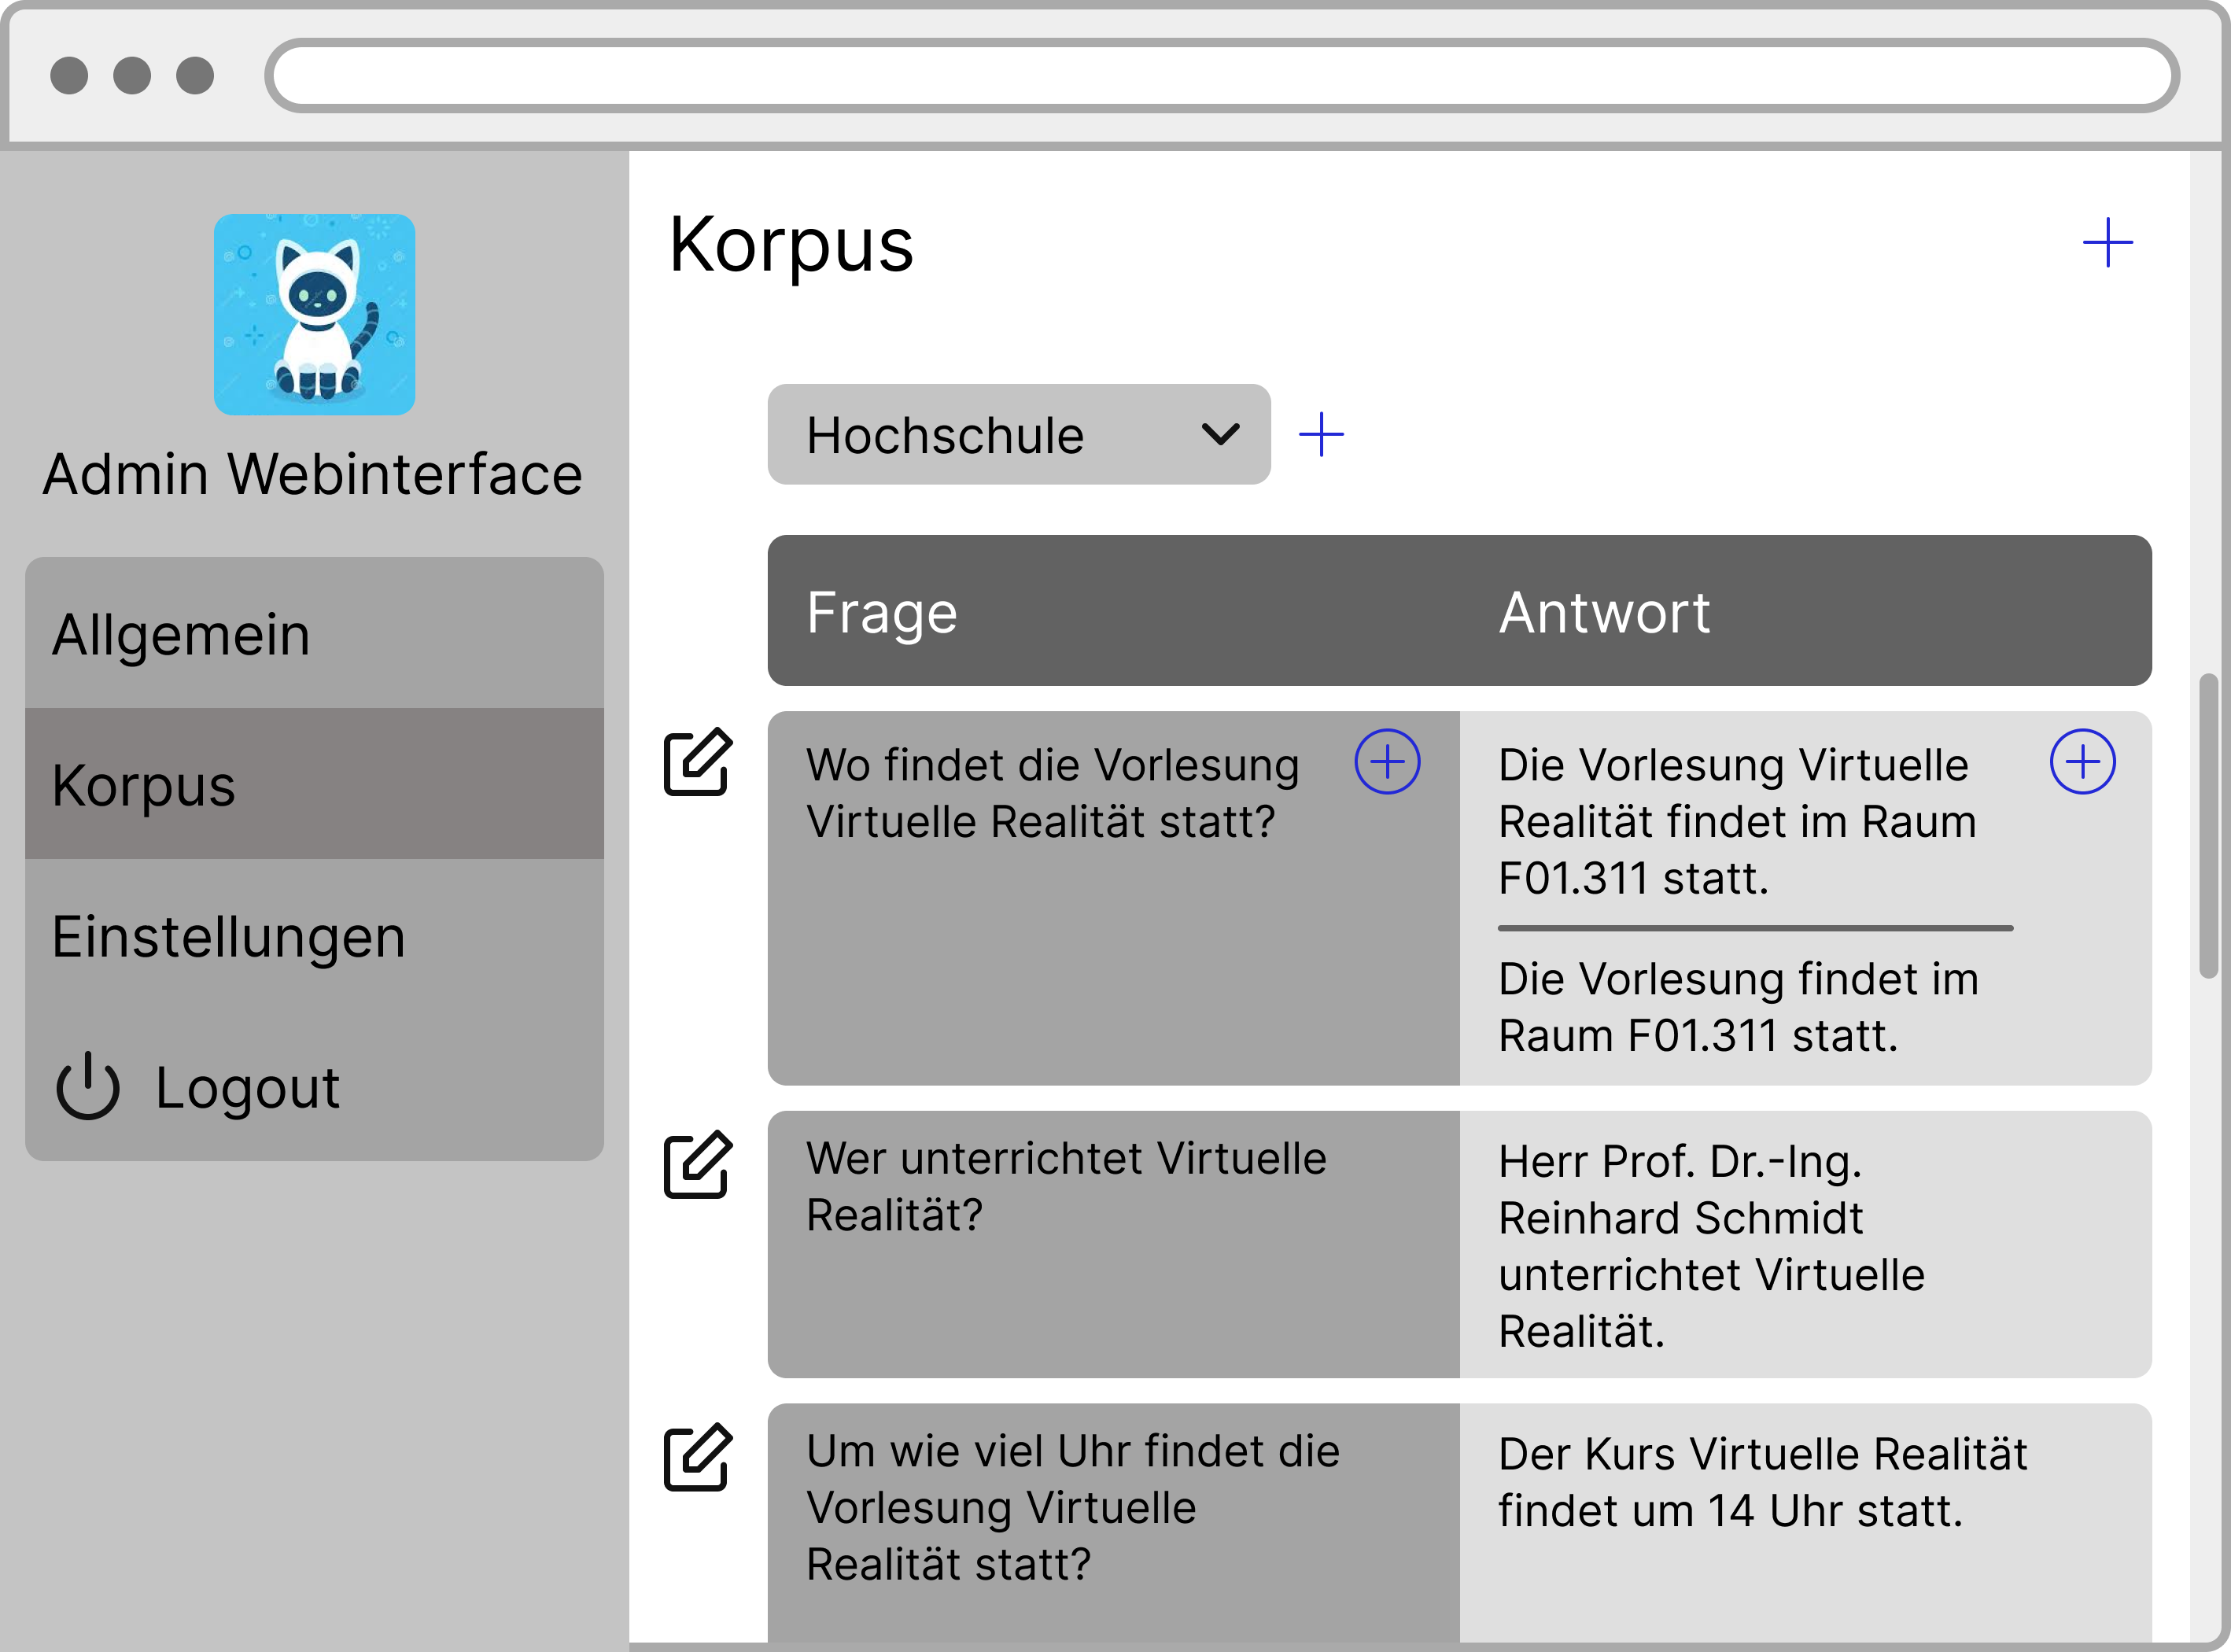
\includegraphics[width=\linewidth]{bilder/new vers. UI Design/Korpus/Admin Interface 02.png} & \textbf{Admin Webinterface: Korpus 02} \newline
    So kann man wie im Beispiel eine weitere Antwort zu der Frage: "Wo findet die Vorlesung Virtuelle
    Realität statt?", hinzufügen.
\end{tabular}

\begin{tabular}{C{6cm}  L{7cm}}
    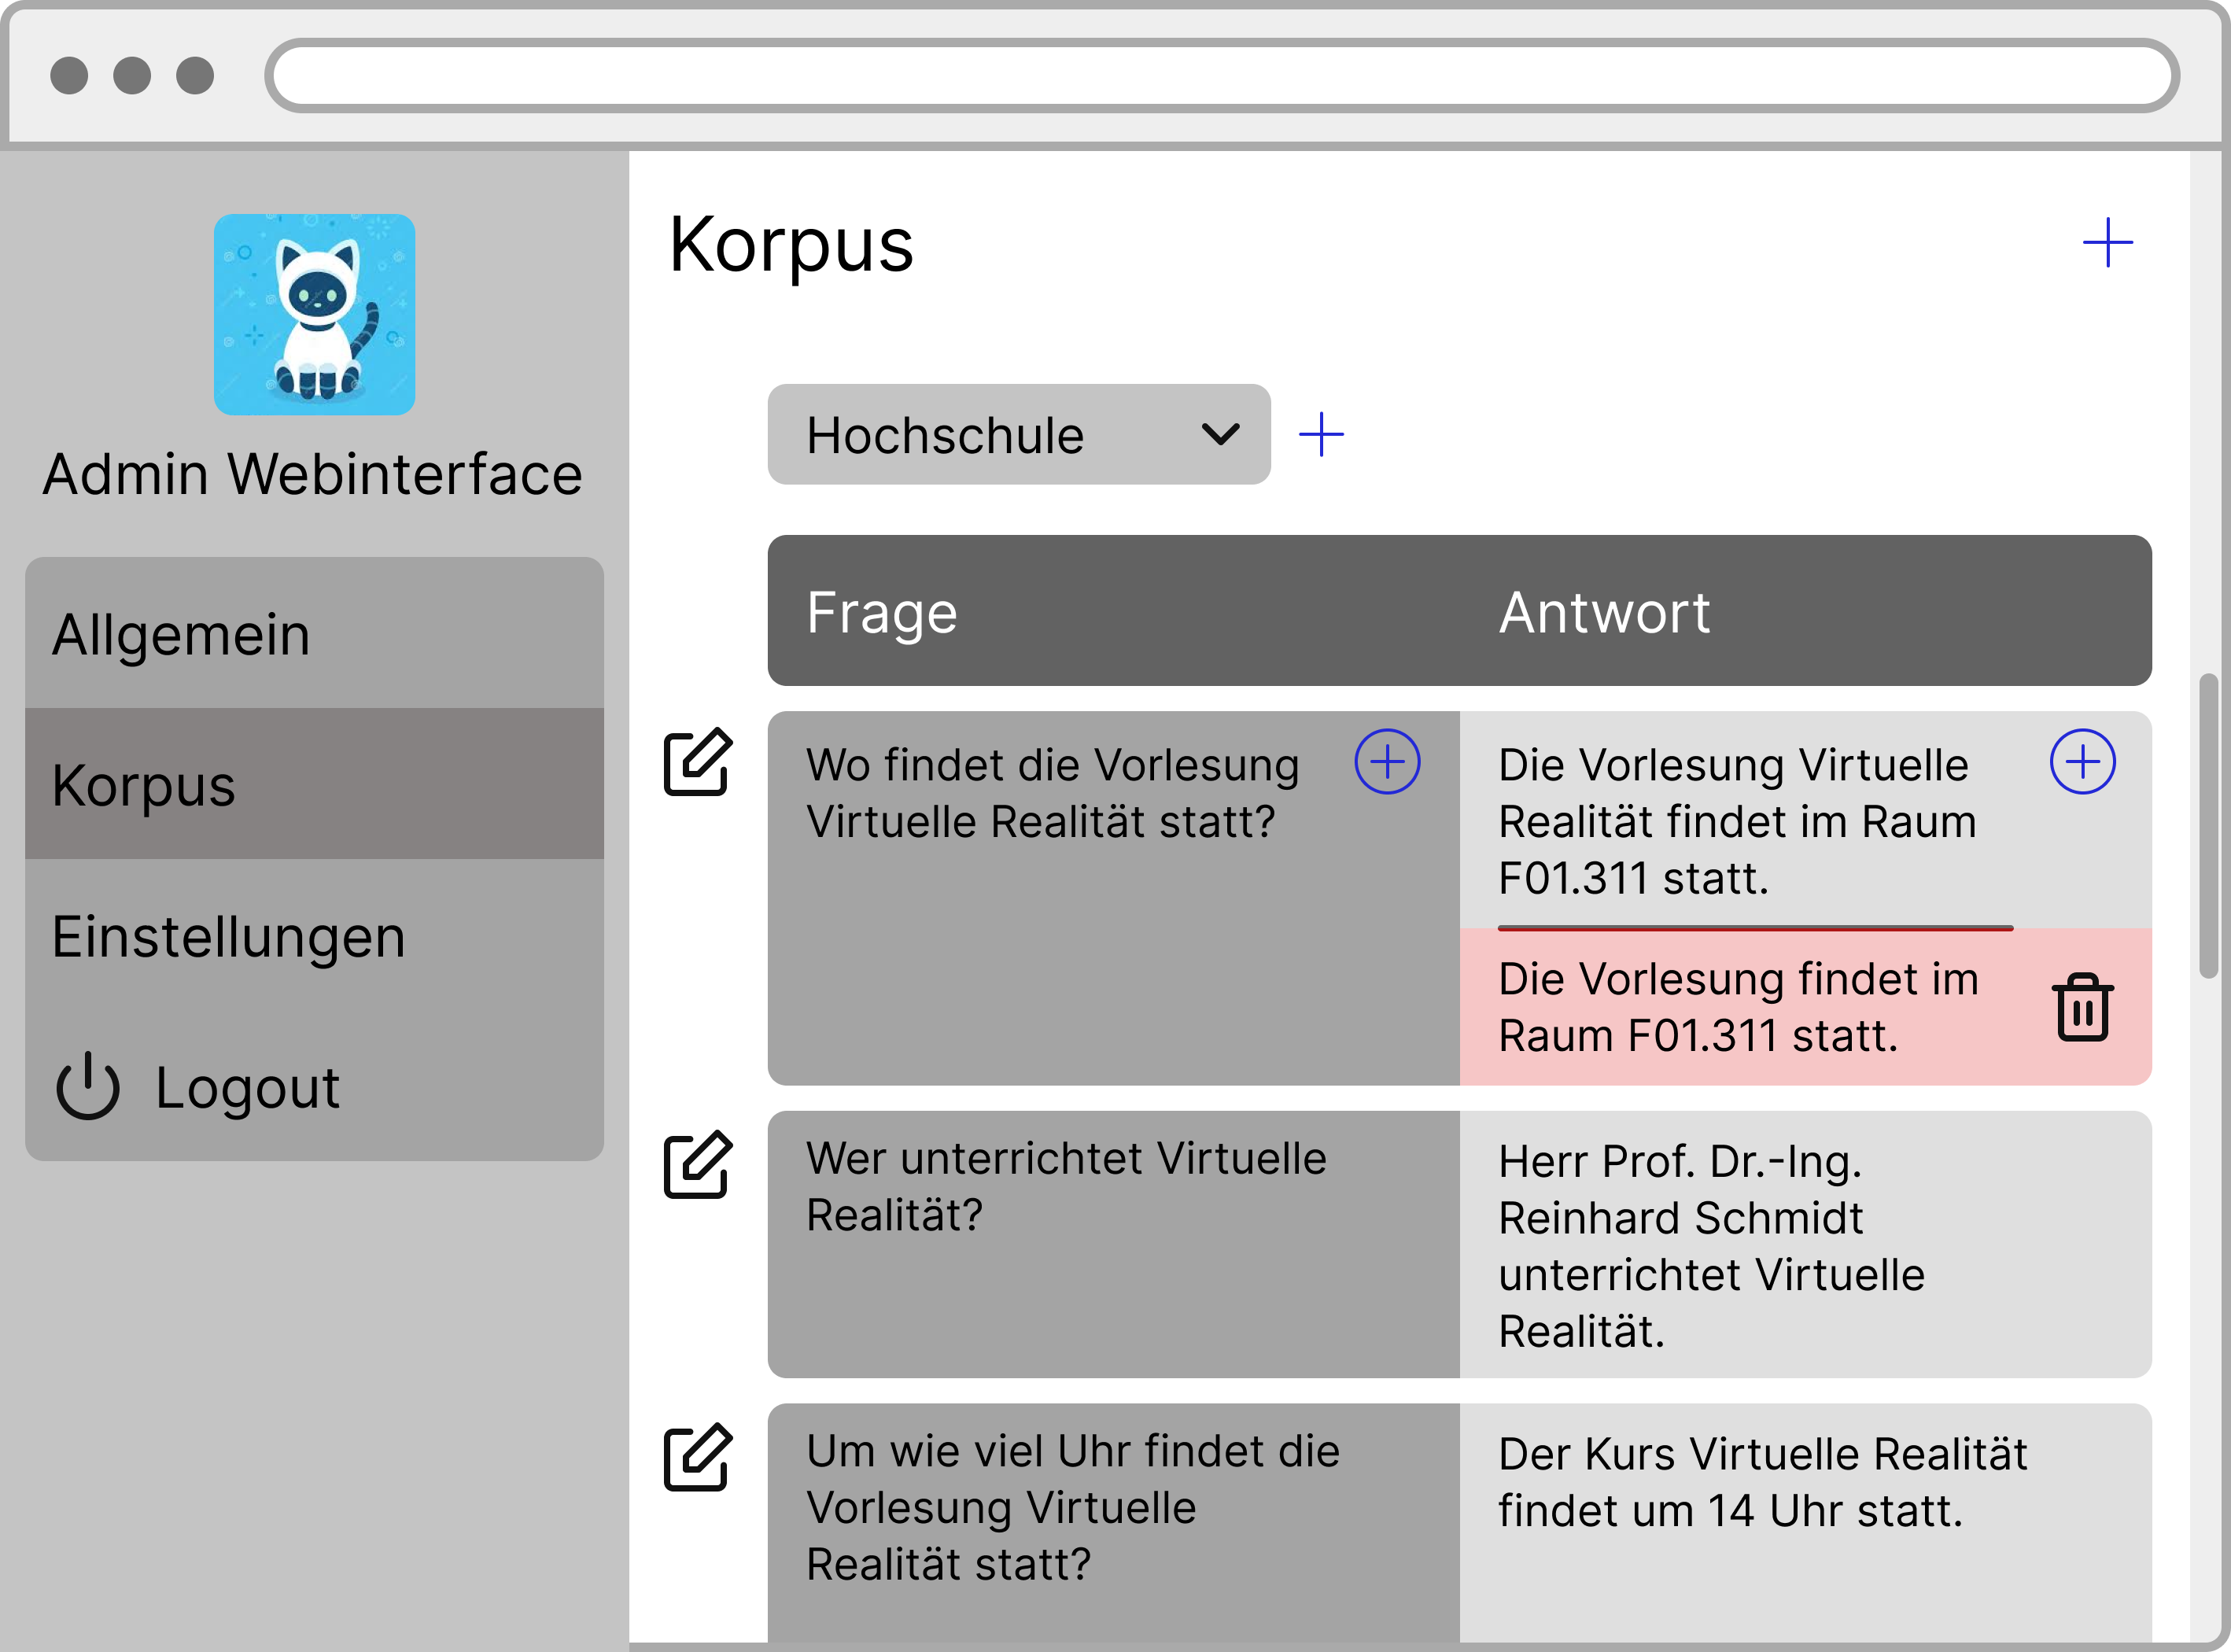
\includegraphics[width=\linewidth]{bilder/new vers. UI Design/Korpus/Admin Interface 03.png}       & \textbf{Admin Webinterface: Korpus 03} \newline
    Natürlich kann man auch die hnzugefügte Antwort entfernen. Man klickt auf das Feld und das Feld erscheint rötlich und ein
    Mülleimersymbol entsteht. Wenn man jetzt auf das Eimer-Symbol klickt kann man die
    Antwort löschen.                                                                                                                                         \\
    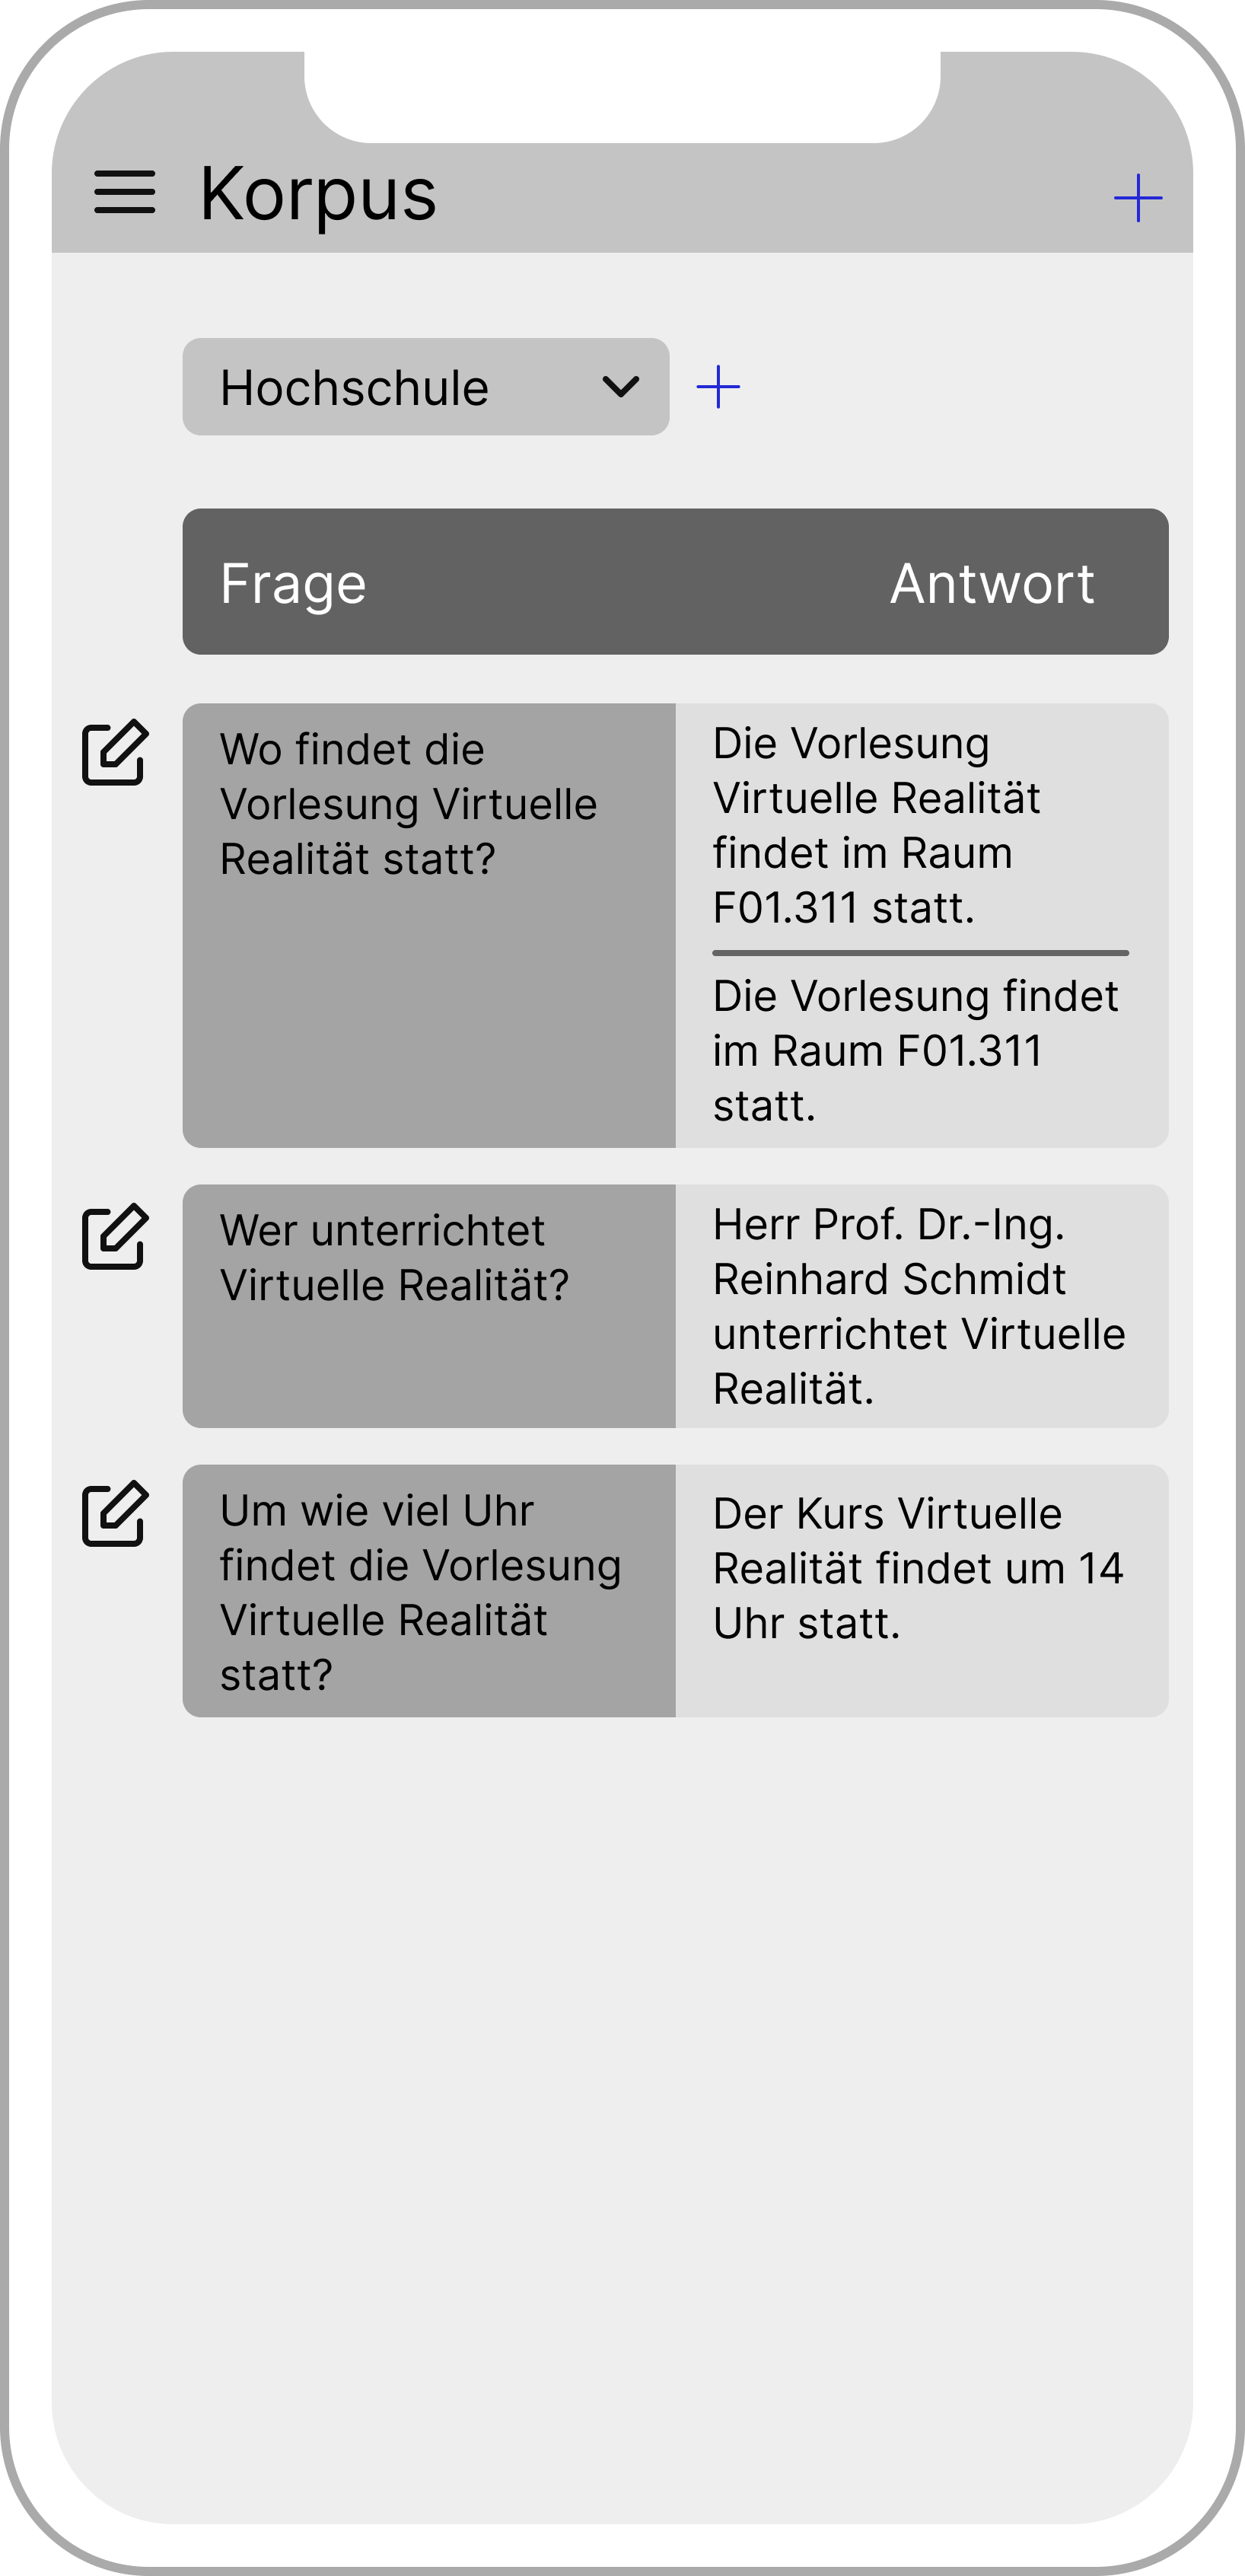
\includegraphics[width=5cm,height=8.5cm]{bilder/new vers. UI Design/Korpus/iPhone X Korpus I.png}  & \textbf{Admin Webinterface mobil: Korpus} \newline
    In der mobilen Version des Korpuses kann man die Elemente genauso editieren wie im Webbrowser.                                                           \\
    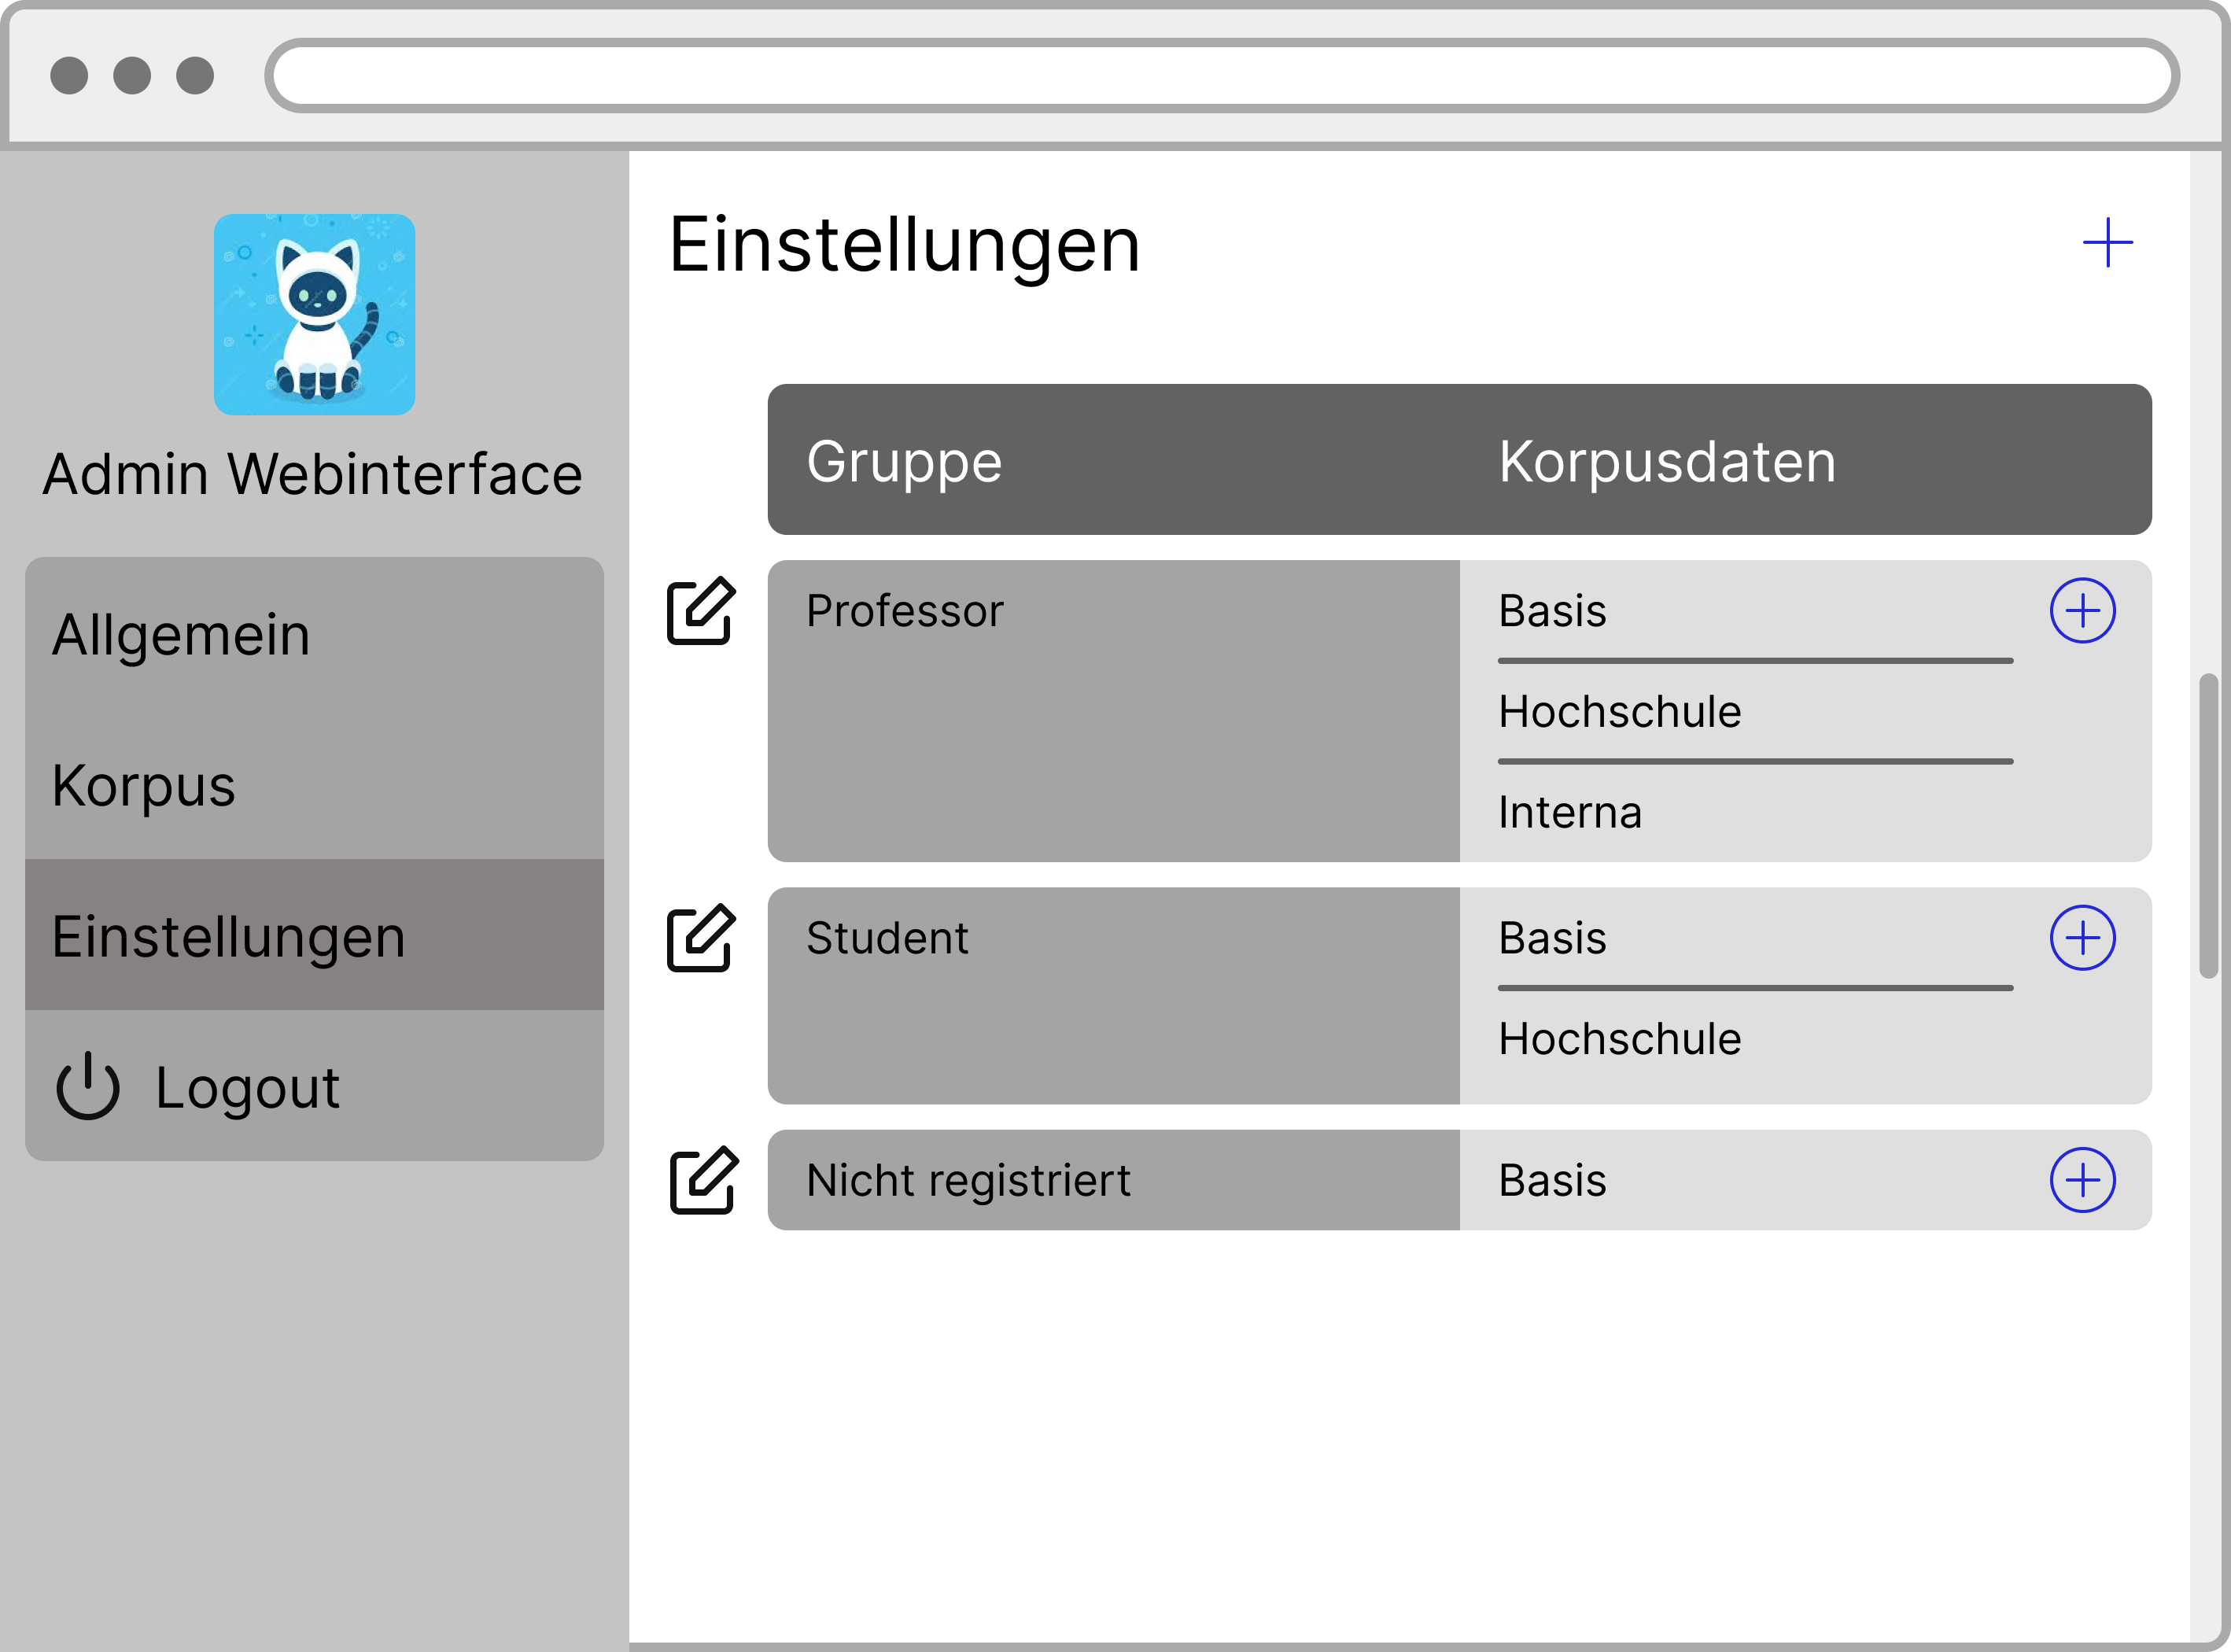
\includegraphics[width=\linewidth]{bilder/new vers. UI Design/Einstellungen/Einstellungen (1).png} & \textbf{Admin Webinterface: Einstellungen} \newline
    In Einstellungen kann der Admin seine Gruppen einsehen, hinzufügen und entfernen. Er kann auch
    die dazugehörenden Korpusdaten sehen und bearbeiten. In den Korpusdaten sind die Domänen der jeweilligen Gruppe eingetragen.
\end{tabular}

\begin{tabular}{C{6cm}  L{7cm}}
    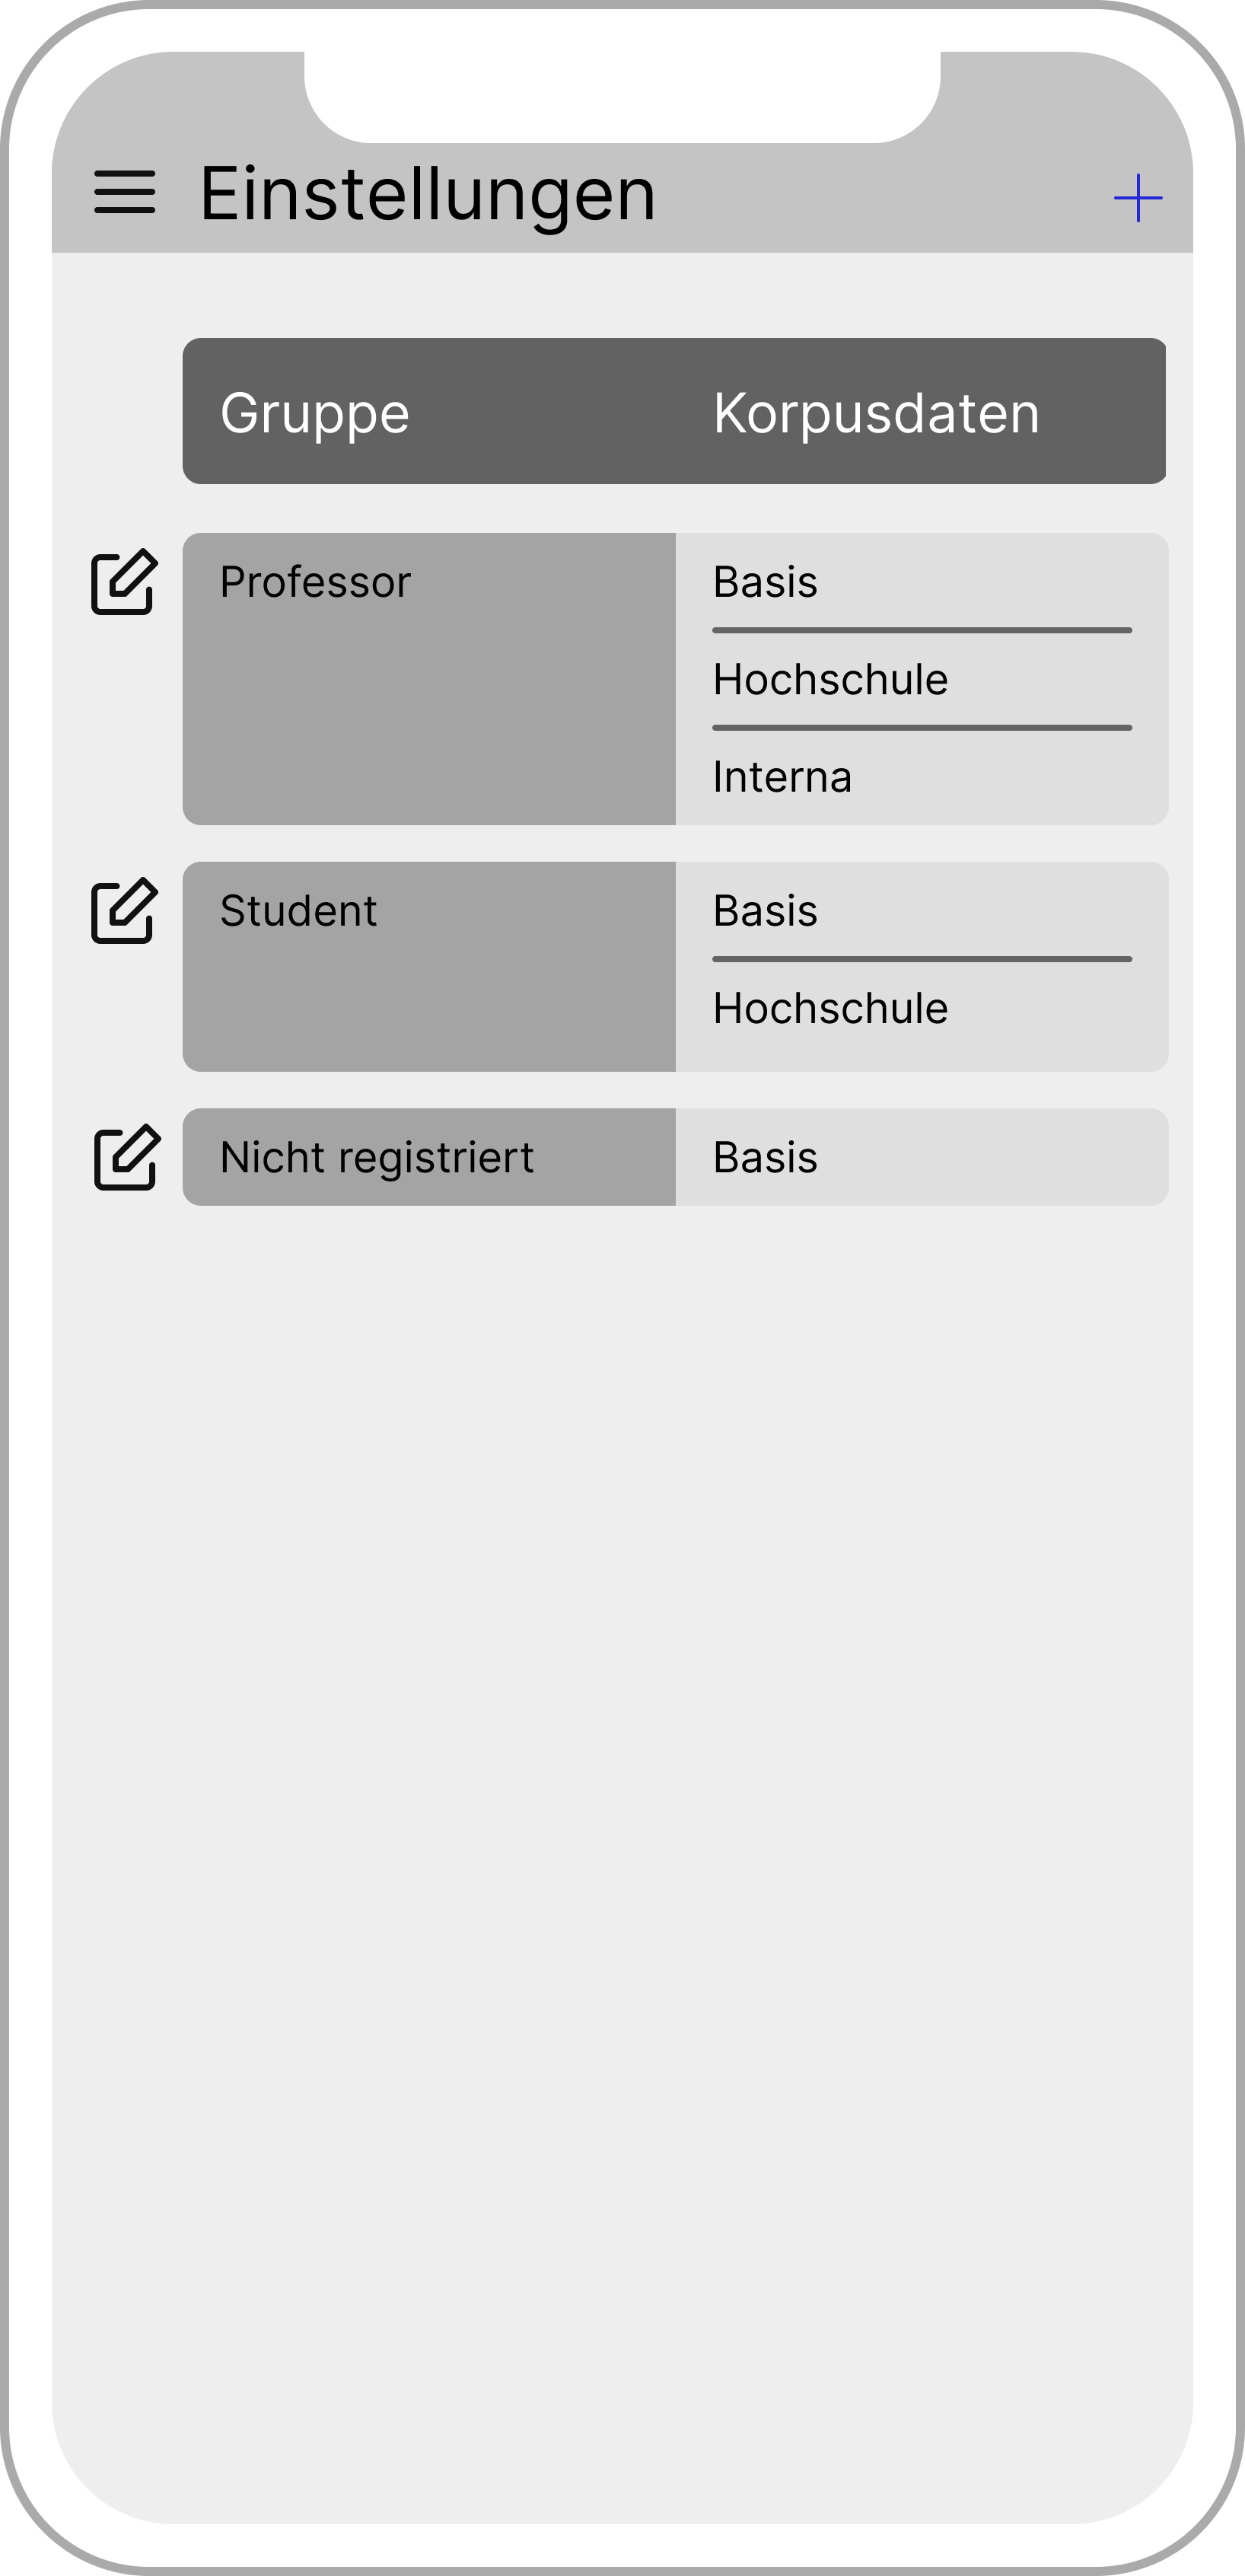
\includegraphics[width=5cm,height=8.5cm]{bilder/new vers. UI Design/Einstellungen/iPhone X Einstellungen I (1).png} & \textbf{Admin Webinterface mobil: Einstellungen} \newline
    In der mobilen Version kann man ebenso die gleichen Features nutzen.                                                                                                             \\
    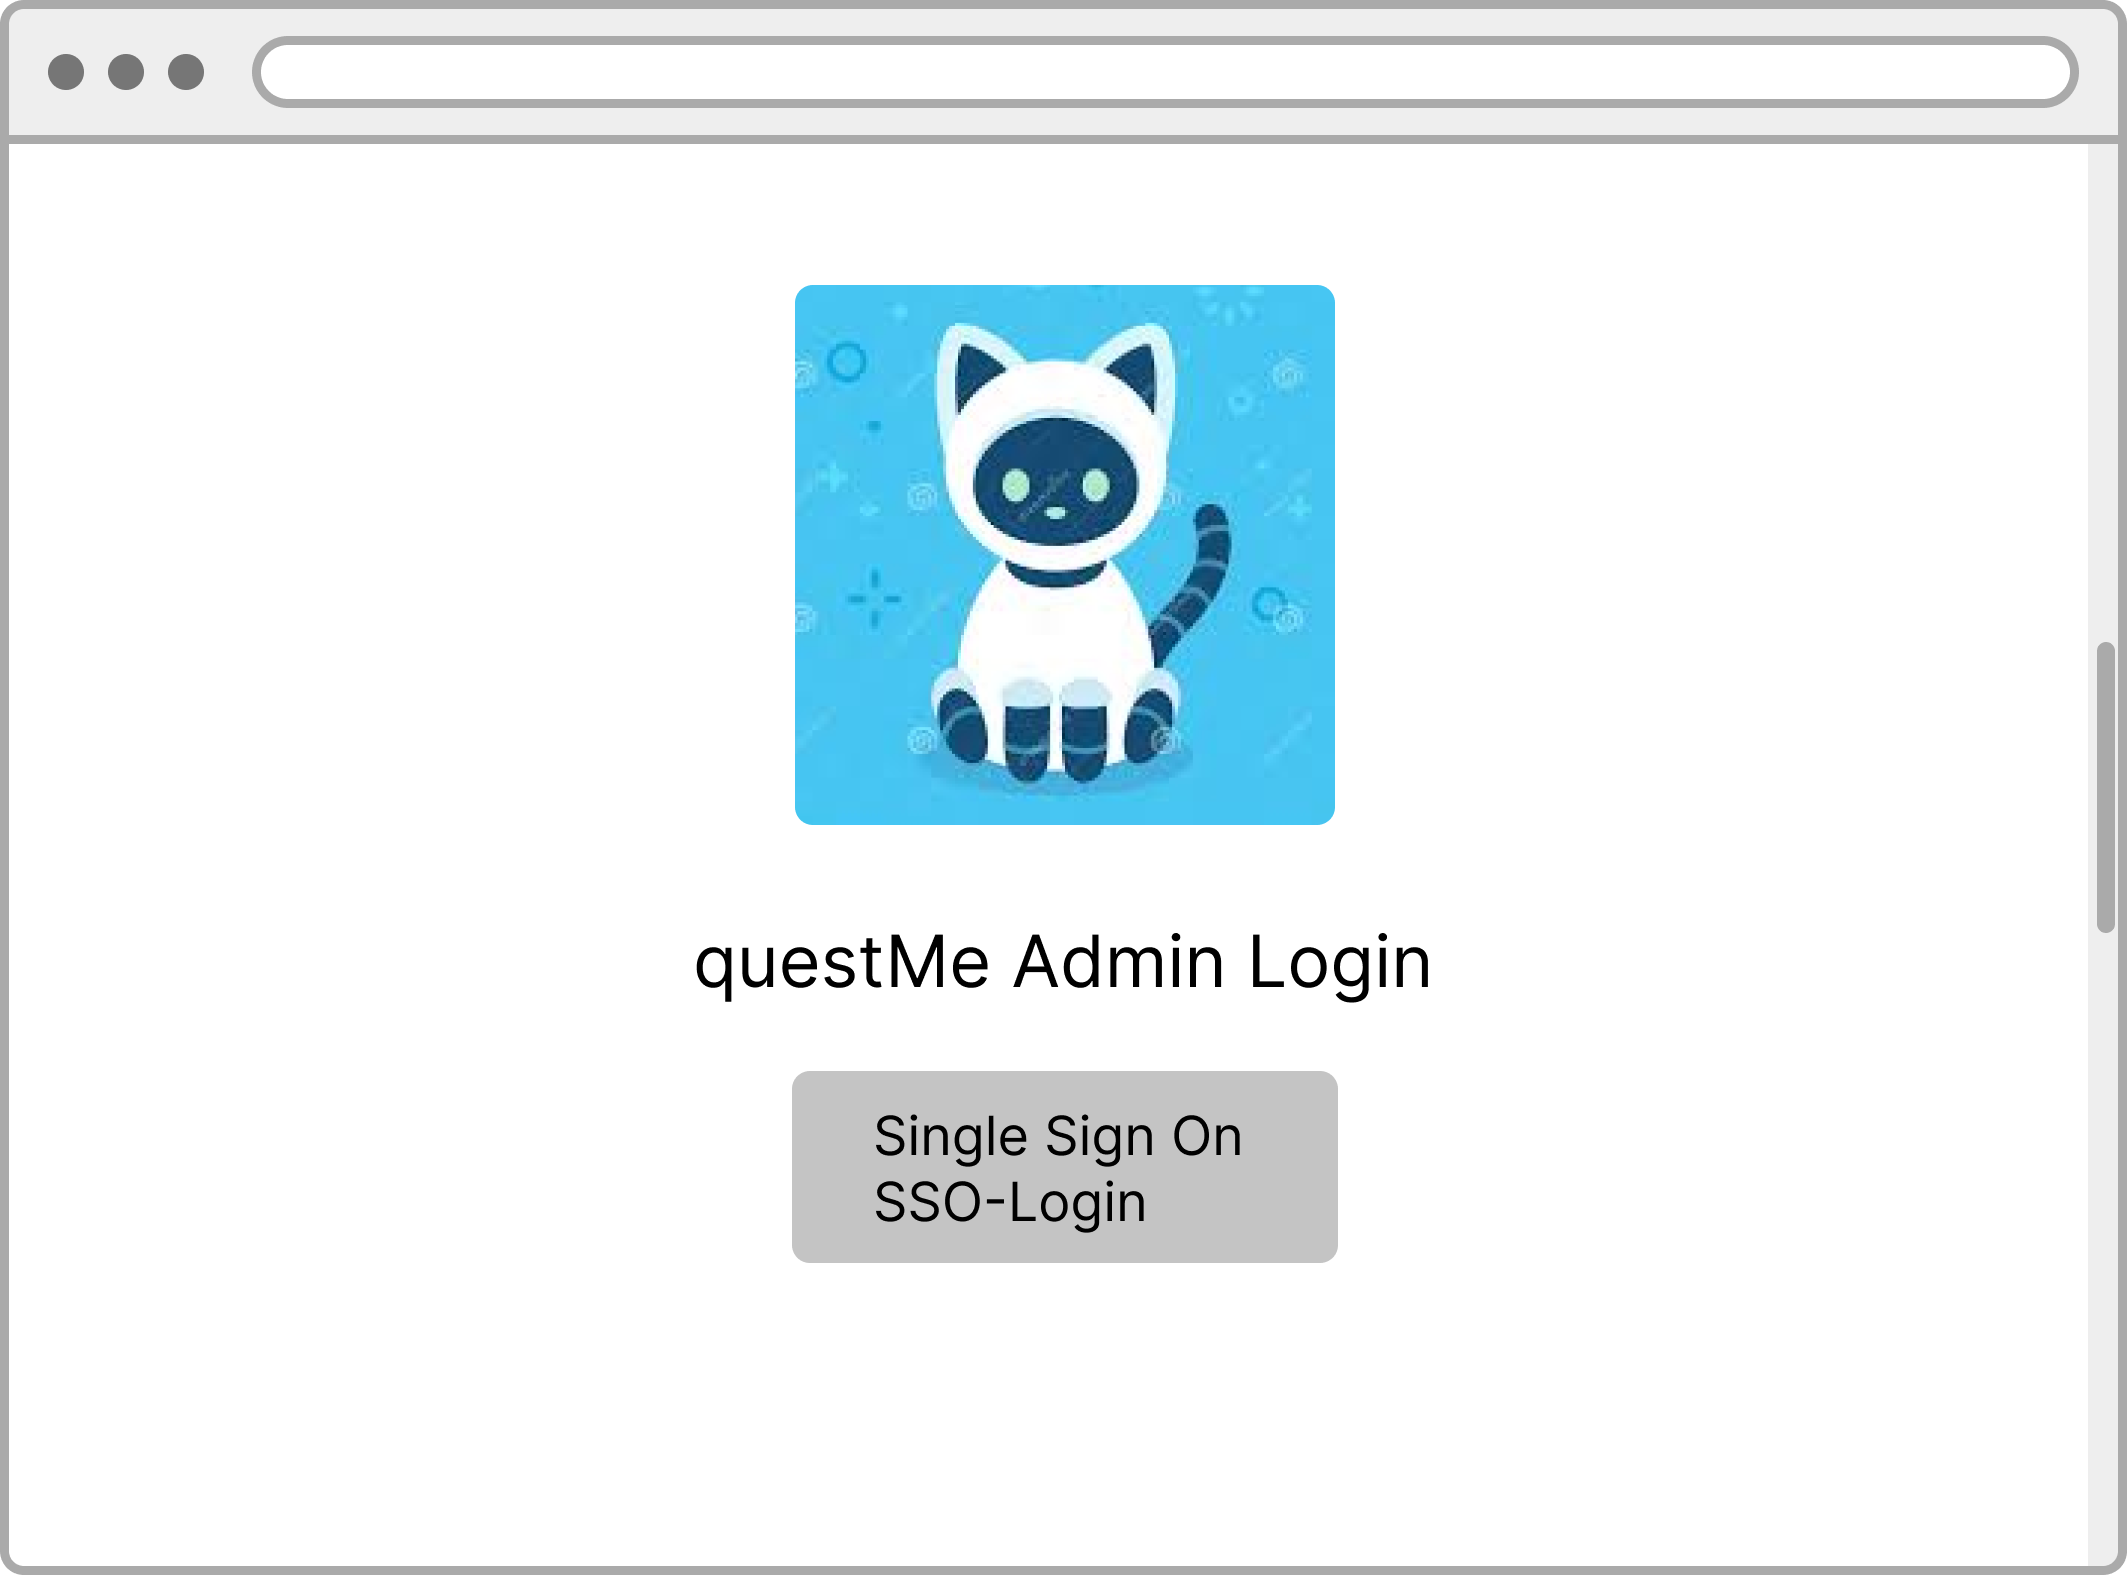
\includegraphics[width=\linewidth]{bilder/new vers. UI Design/Login SSO/Admin Interface SSO.png}                    & \textbf{Admin Webinterface: Single Sign On} \newline
    Mit einem Link gelangt der Admin zu der Admin Login Seite, wo er mit Shibboleth sich einloggen kann.                                                                             \\
    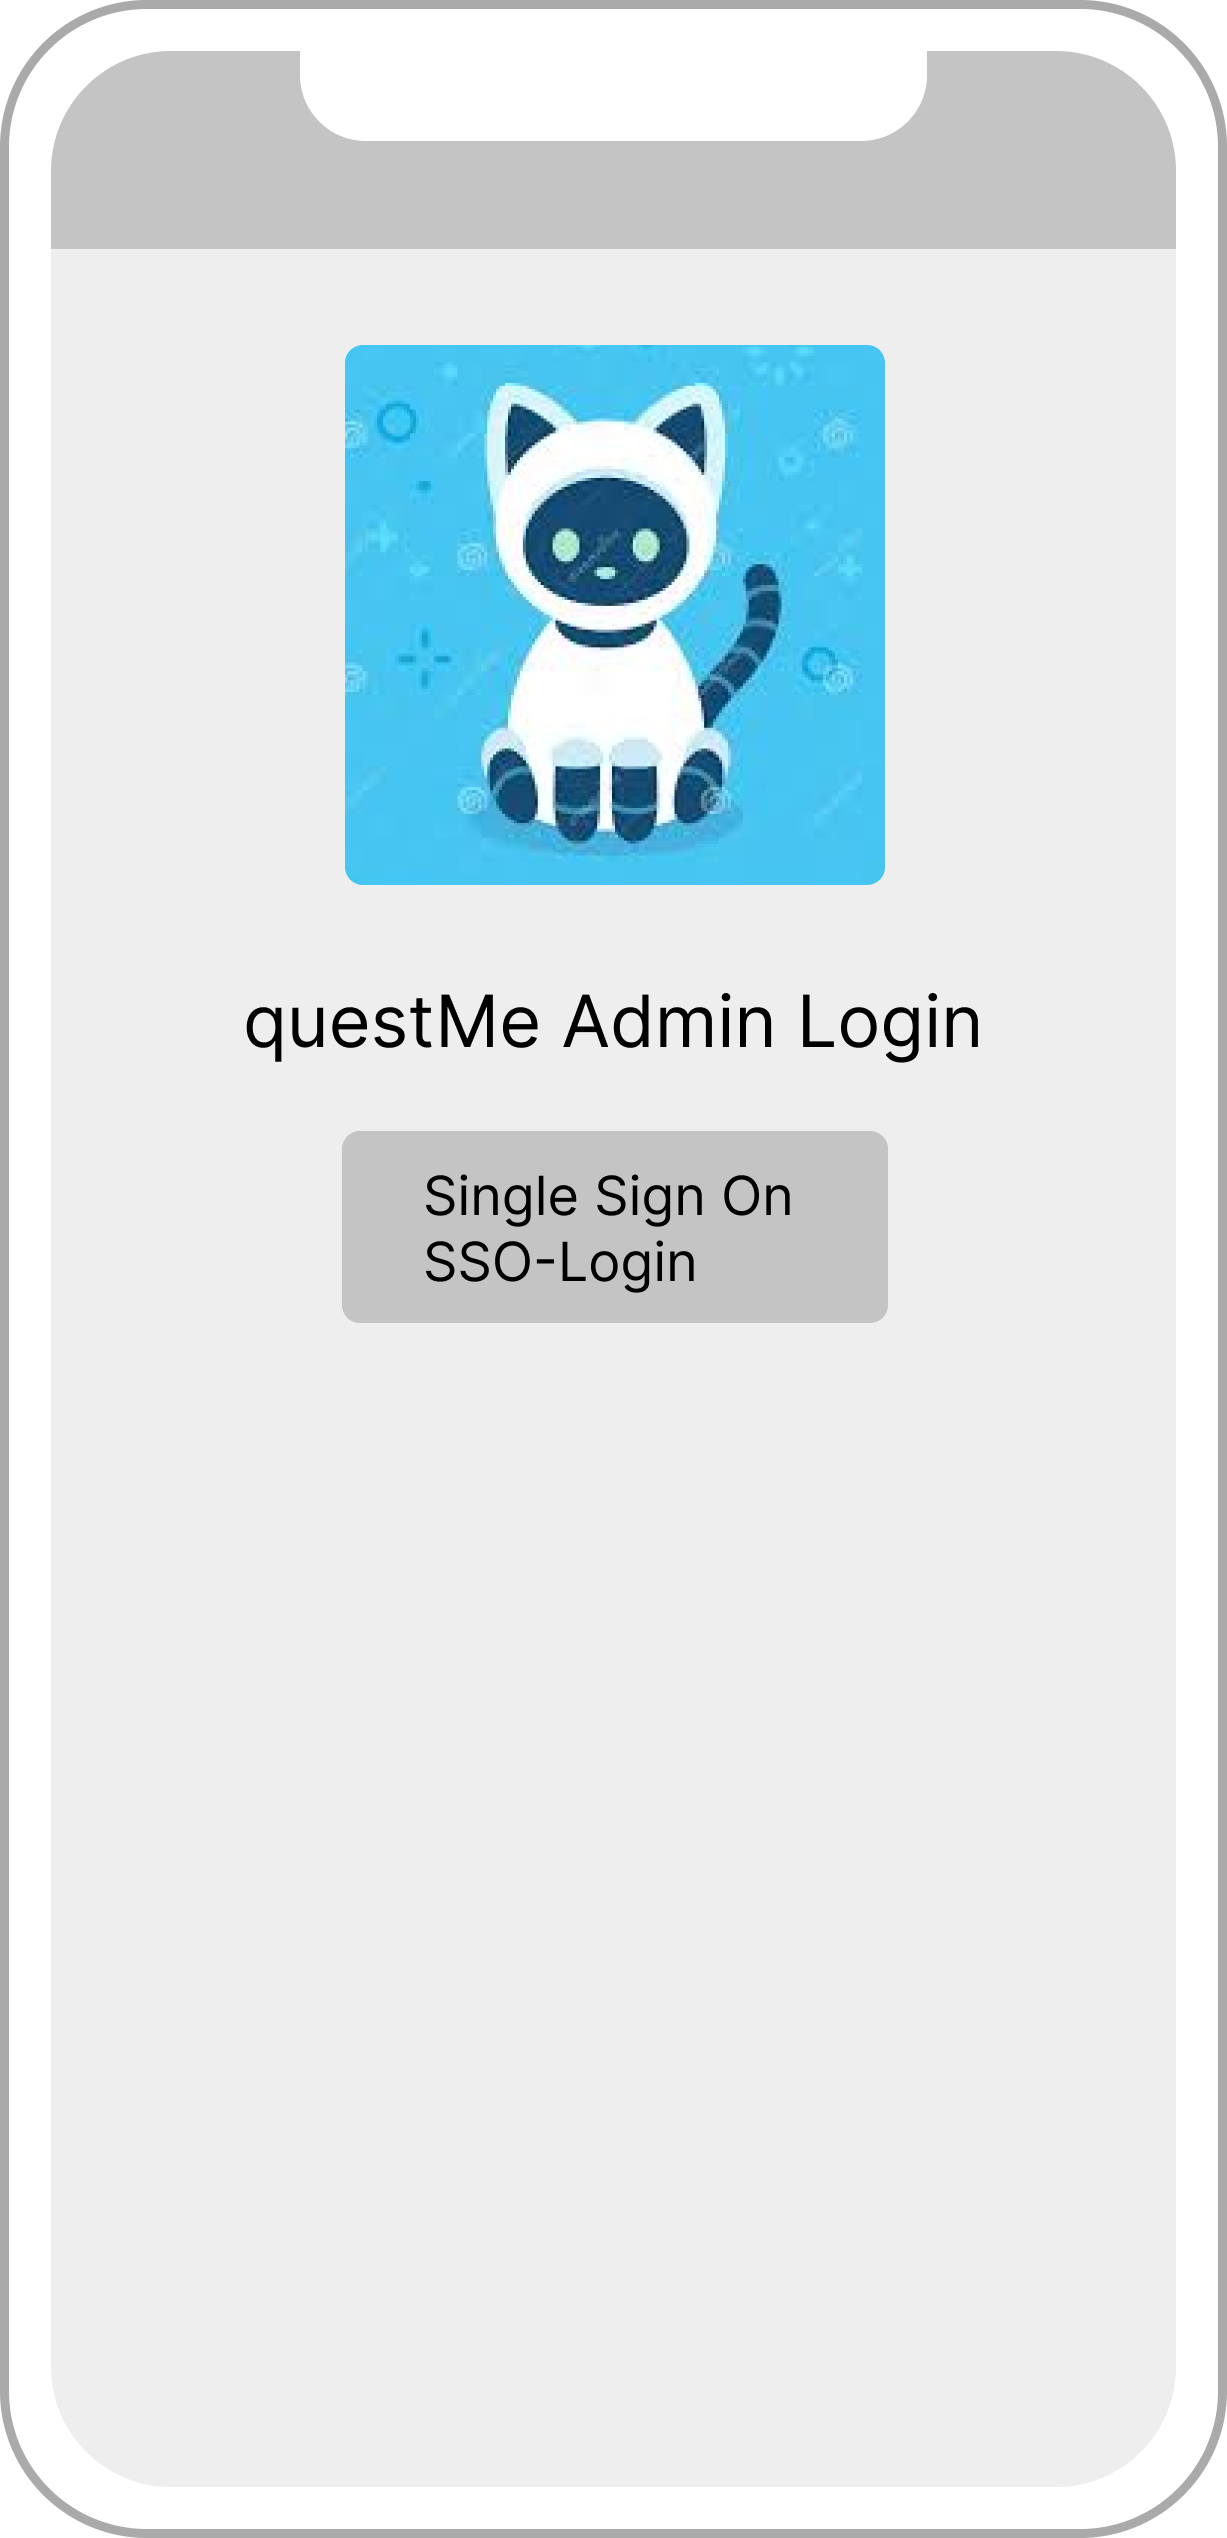
\includegraphics[width=5cm,height=8.5cm]{bilder/new vers. UI Design/Login SSO/Interface SSO v1.2.png}               & \textbf{Admin Webinterface mobil: Single Sign On} \newline
    In der mobilen Version wird die gleiche Prozedur benutzt.
\end{tabular}

\newpage

\subsection{Version 1}

Das sind die älteren Entwürfe des Designs. Bei diesen Entwürfen haben wir uns nur auf die Struktur
konzentriert und eine grobe Version erstellt. Uns war es hier hauptsächlich wichtig
die Ideen, die wir durch die Recherche aufgenommen haben zu projezieren.
\\

\begin{tabular}{C{6cm}  L{7cm}}
    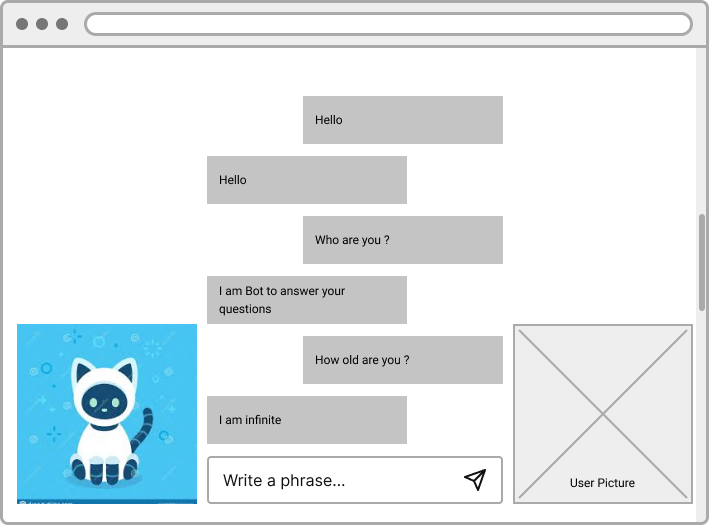
\includegraphics[width=\linewidth]{bilder/old vers. UI Design/WebChat.png}                   & \textbf{Webchat} \newline
    In der alten Version unseres Webchat designs haben wir gedacht, auch für den
    Nutzer ein Profilbild hinzu zufügen. Diese Idee aber schien zu aufwendig zu sein und wir versuchen
    zuerst ein Minimal Virable Product zu erschaffen.                                                                                           \\
    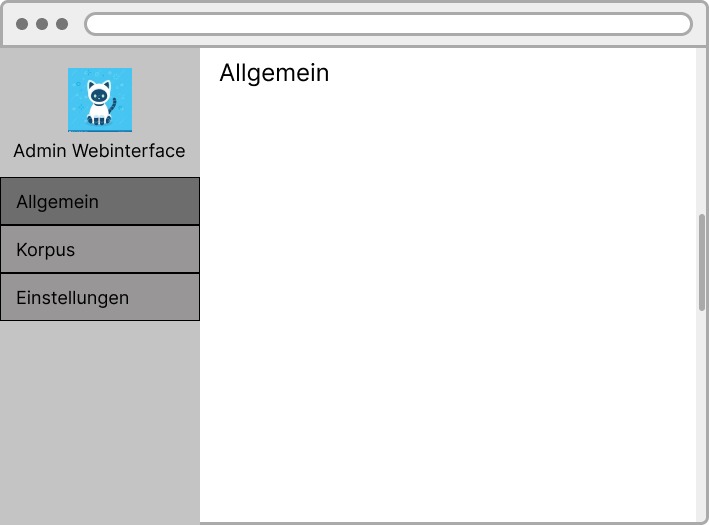
\includegraphics[width=\linewidth]{bilder/old vers. UI Design/Admin Interface Allgemein.png} & \textbf{Admin Interface: Allgemein} \newline
    Im Admin Interface kann man auf der linken Seite das Menü sehen. Was aber hier fehlt ist der Logout Button.
    Wir hatten auch keine richtigen Vorstellungen, was wir einführen möchten.                                                                   \\
    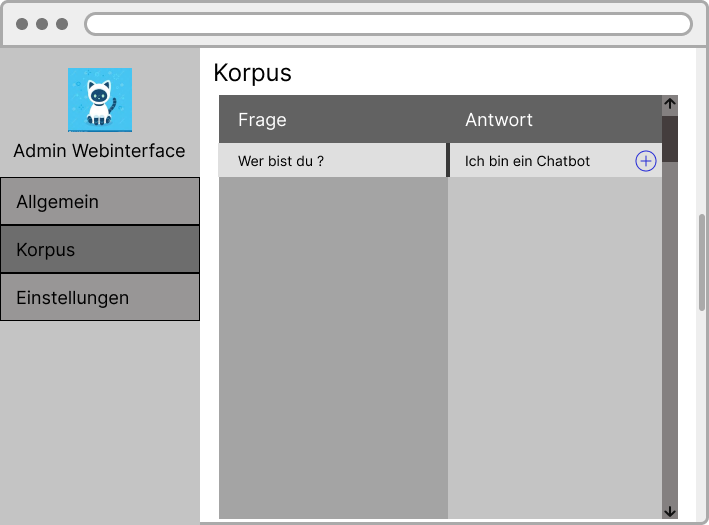
\includegraphics[width=\linewidth]{bilder/old vers. UI Design/Admin Interface (1).png}       & \textbf{Admin Interface: Korpus 00} \newline
    Im Korpus wollten wir schon von Anfang an das Hinzufügen darstellen, wussten aber nicht
    wie und habe herumprobiert.
\end{tabular}

\begin{tabular}{C{6cm}  L{7cm}}
    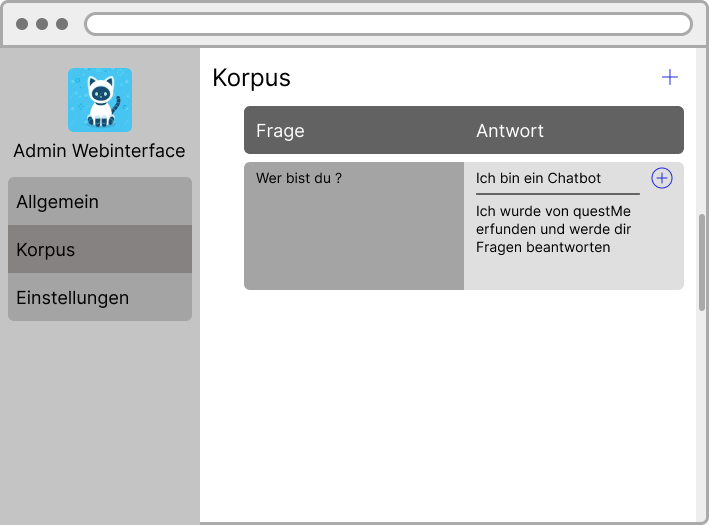
\includegraphics[width=\linewidth]{bilder/old vers. UI Design/Admin Interface I.png}  & \textbf{Admin Interface: Korpus 01} \newline
    In diesem Beispiel sieht man ein Basisbeispiel mit einer Frage die im Alltag gestellt wird und die dazugehörenden Antworten. Wie wir diese aber
    editieren haben wir hier noch nicht gezeigt.                                                                                           \\
    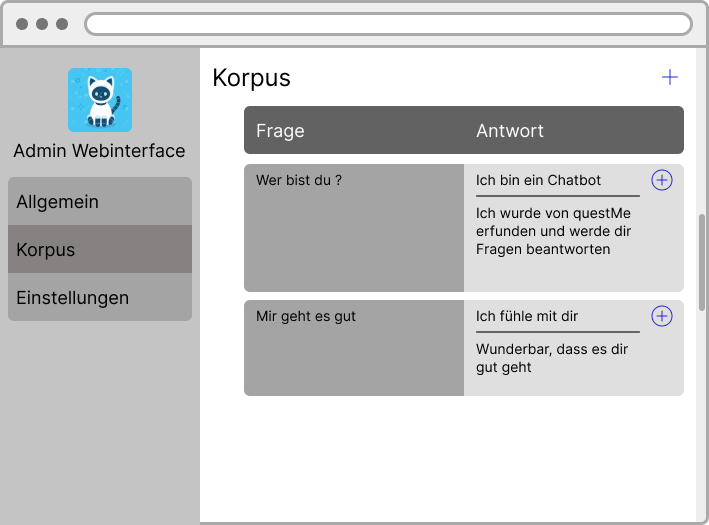
\includegraphics[width=\linewidth]{bilder/old vers. UI Design/Admin Interface II.png} & \textbf{Admin Interface: Korpus 02} \newline
    Im nächsten Beispiel sieht man eine weitere Frage und die dazugehörenden zwei Antworten. Es ist immer noch nicht
    bekannt, wie man Antworten und Fragen editiert oder Fragen und Antworten von verschiedenen Domänen bearbeitet.                         \\
    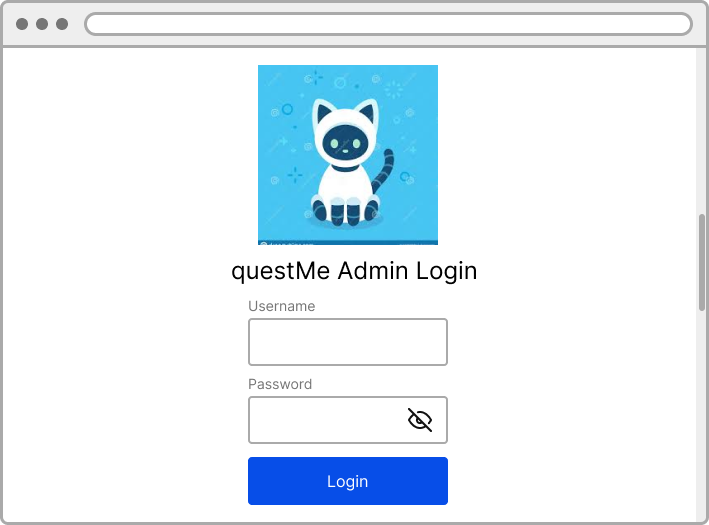
\includegraphics[width=\linewidth]{bilder/old vers. UI Design/Admin Interface.png}    & \textbf{Admin Interface: Admin Login} \newline
    Hier haben wir nur einen klassischen Login Eingabefeld dargestellt, weil wir uns nicht klar waren, wie es mit der Athentifizierung und dem Admin
    Login funktioniert.
\end{tabular}


\subsection{Kriterien für Usability}
Unsere Kriterien für Usability, die uns wichtig sind und für und unser User Interface
essentiell sind, werden wir hier kurz erläutern.
\newline

\noindent\textbf{1.Responsive Webdesign}

\noindent Wir möchten unseren ChatBot auf allen Geräten ohne Probleme ausführen lassen.
Das heißt, dass wir auch auf mobilen Geräten unsere Software im Browser laufen lassen wollen.
Die mobile Seite sollte dann auch auf die wichtigsten Elemente beschränkt werden, damit
der Benutzer es leichter hat die Icons treffsicher mit ihren Fingern zu benutzen.
\newline

\noindent\textbf{2.Gute Lesbarkeit}

\noindent Unsere Anwendung sollte leicht zu lesen sein, weil das Lesen auf dem Bildschirm
grundsätzlich schwieriger ist. Deswegen sollten wir auf jeden Fall
auf Textgröße und Kontrastreiche Farben achten.Die Textgröße sollte mindestens
12pt haben. Auch sollten wir lange Textblöcke und
Schachtelsätze vermeiden.
\newline

\noindent\textbf{3.Gute Navigation}

\noindent Eine übersichtliche und eine verständliche Navigation ist das wichtigste bei einer Webseite.
Eine gute Navigation verhindert Verwirrung und Unterstützt den Benutzer zu seinem Ziel zu gelangen.
Bei der Navigation sollte man darauf achten, dass alle Verlinkungen funktionieren.
\newline

\noindent\textbf{4.Schnelle Ladezeiten}

\noindent Die Webseite sollte ihre Inhalte schnell laden und keine großen Verzögerungen
aufzeigen. Sie sollte bei ungefähr drei Sekunden liegen, um keine User zu verlieren.
\newline

\noindent\textbf{5.Interessantes Design}

\noindent Eine Konsistente Einhaltung von bestimmten Farben ist sehr wichtig. Der erst Eindruck von
einer Webseite zeigt schon, ob die User die Webseite benutzen möchten oder nicht.
So können Benutzer durch Bilder mit schlechter Qualität oder zu grellen Farben abgeschreckt werden.
Pop-Ups sollten in Grenzen gehalten werden oder vermieden werden.

\subsection{Usability Test}
Hier beschreiben wir welche Methode wir zum Testen unserer Usability Kriterien benutzen
möchten.
\newline

\noindent \textbf{Remote User Testing}

\noindent Zuerst plannen wir was wir testen möchten und dann wie wir testen möchten. In unserem Fall haben wir uns
für remote testing entschieden. Als nächstes überlegen wir uns besondere Tasks, die der User absolvieren muss, um
zu erkennen, ob unsere Kriterien eingehalten werden und was wir Verbessern sollten.
Die Szenarien sollten so einfach und realistisch sein, dass der Benutzer es leicht durchführen kann.
Dann müssen wir auch Tester finden, welche in unserer Zielgruppe passen.


